\documentclass{book}
\usepackage{amssymb,amsmath,mathtools}


\usepackage{algorithm2e,algorithmic}

\usepackage{mathrsfs}
\usepackage{paralist}

\usepackage{esint} % for \fint

\allowdisplaybreaks

\usepackage{color}		% enable color characters
\usepackage{graphicx} 	% insert image files
\usepackage{enumerate} 	% enumerate items
\usepackage{caption}
\usepackage{subcaption}
\usepackage{multirow,multicol}
\usepackage[makeroom]{cancel}

\usepackage[colorlinks=true,linkcolor=blue,citecolor=blue]{hyperref}

\usepackage{makeidx}

\newcommand{\cem}[1]{\color{magenta}{\em{#1}}} % color emphasize
\newcommand{\dual}[2]{{#1}^{(#2)}} % color emphasize

\newcommand{\tr}{{\mathrm{tr}}}
\renewcommand{\vec}{{\mathrm{vec}}}

\newcommand{\dd}{{\,\mathrm{d}\,}}
%%
%% horizontal and vertical centering in table p mode
%%
\usepackage{array}
\newcolumntype{P}[1]{>{\centering\arraybackslash}p{#1}} % horizontal centering
\newcolumntype{M}[1]{>{\centering\arraybackslash}m{#1}} % vertical centering

%%
%% define bold font for the alphabet
%%
\usepackage{pgffor}
\foreach \letter in {a,...,z}{ % bold font for a..z
\expandafter\xdef\csname \letter \endcsname{\noexpand\ensuremath{\noexpand\mathbf{\letter}}}
}
\foreach \letter in {A,...,Z}{ % bold font for A..Z
\expandafter\xdef\csname \letter \endcsname{\noexpand\ensuremath{\noexpand\mathbf{\letter}}}
}
\foreach \letter in {A,...,Z}{ % `field' font for AA..ZZ
\expandafter\xdef\csname \letter\letter \endcsname{\noexpand\ensuremath{\noexpand\mathcal{\letter}}}
}
\foreach \letter in {A,...,Z}{ % `field' font for AAA..ZZZ
\expandafter\xdef\csname \letter\letter\letter \endcsname{\noexpand\ensuremath{\noexpand\mathbb{\letter}}}
}
\newcommand{\balpha}{{\boldsymbol{\alpha}}}
\newcommand{\bbeta}{{\boldsymbol{\beta}}}
\newcommand{\bgamma}{{\boldsymbol{\gamma}}}
\newcommand{\bkappa}{{\boldsymbol{\kappa}}}
\newcommand{\bmu}{{\boldsymbol{\mu}}}
\newcommand{\btheta}{{\boldsymbol{\theta}}}
\newcommand{\bTheta}{{\boldsymbol{\Theta}}}
\newcommand{\bPi}{{\boldsymbol{\Pi}}}
\newcommand{\bSigma}{{\boldsymbol{\Sigma}}}
\newcommand{\bPhi}{{\boldsymbol{\Phi}}}
\newcommand{\bLambda}{{\boldsymbol{\Lambda}}}
\newcommand{\bdeta}{{\boldsymbol{\eta}}}
\newcommand{\bphi}{{\boldsymbol{\phi}}}



%%
%% add definitions and theorems
%%
\usepackage[thmmarks,amsmath]{ntheorem}
\theorembodyfont{\normalfont}
\newtheorem{deff}{Definition}[section]
\newtheorem{thm}{Theorem}[section]
\newtheorem{prop}{Proposition}[section]
\newtheorem{lem}{Lemma}[section]
\newtheorem{cor}{Corollary}[section]
\newtheorem{rmk}{Remark}[section]
\newtheorem{alg}{Algorithm}[section]
\newtheorem{ex}{Example}[section]
\newtheorem{ques}{Question}[section]
\newtheorem{ans}{Answer}[section]
\newtheorem{prob}{Problem}[section]
\newtheorem{sol}{Solution}[section]
\newtheorem*{prof}{Proof}[section] 

\title{Quantitative Finance Handbook}
\author{Xi Tan (xtan3.1415926@gmail.com)}

\makeindex

\begin{document}

\maketitle
\tableofcontents
\chapter*{Preface}
This book project, which consists of four subjects: Finance, Mathematics, Statistics, and Computer Science, is tailored specifically to prepare someone for a quant career. It originated from my general belief of the hierarchy of solving a problem --- problems are solved at strategic, tactical, and operational levels.

{\em{Microeconomics}} and {\em{Macroeconomics}} explain the driving forces of capital markets, from a legislator's perspective. {\em{Accounting}} and {\em{Corporate Finance}} take a closer and necessary look at these forces, from a different angle. {\em{Stochastic Calculus}} and {\em{Asset Pricing}} provide with a set of tools and ideas that enables us to {\bf{strategically}} model one of the central problems in Quantitative Finance.

Generally speaking, there are two paths to solve a quantitative finance problem at the {\bf{tactical}} level: the mathematical way and the statistical way. There are only two pieces of math we need to know: {\em{Analysis}}, in particular measure-theoretical probability and differential equations; and {\em{Linear Algebra}}, with functional analysis in mind. Statistics, on the other hand, should start with {\em{Statistical Experiment Design}}, from which we learn how to collect data for statistical models. Next, the study of {\em{Random Variables}} and {\em{Stochastic Processes}} introduce the building blocks of the statistical ``pillbox'', with {\em{Mathematical Statistics}} the ``scaffold''. Once the ``pillbox'' is ready, we are equipped to tackle our problems using {\em{Machine Learning}}, which is essentially a collection of statistical models and optimization algorithms.

{\em{Computer Architecture}} and {\em{Operating System}} are respectively about the ``hardware'' and ``software'' of a single computer. The interaction of multiple computers is understood in {\em{Computer Network}}. Once we are comfortable with these concepts, we will be able to use {\em{Data Structure and Algorithms}} to solve problems at the {\bf{operational}} level, and use {\em{C++}} and/or {\em{Java}} to implement our ideas.

I am aware that it can take a while, and even multiple advanced degrees, to finish this curriculum, but let's remember the motto from the Leipzig Gewandhaus Orchestra: ``{\bf{\em{Res severa est verum gaudium}}}''.

\vspace{8mm}
\hfill {\em{Xi Tan}}

\hfill {\em{West Lafayette, IN}}

\hfill {\em{October, 2013}}

\addcontentsline{toc}{chapter}{Preface}

\part{Finance and Economics}
\documentclass{book}
\usepackage{amssymb,amsmath,mathtools}


\usepackage{algorithm2e,algorithmic}

\usepackage{mathrsfs}
\usepackage{paralist}

\usepackage{esint} % for \fint

\allowdisplaybreaks

\usepackage{color}		% enable color characters
\usepackage{graphicx} 	% insert image files
\usepackage{enumerate} 	% enumerate items
\usepackage{caption}
\usepackage{subcaption}
\usepackage{multirow,multicol}
\usepackage[makeroom]{cancel}

\usepackage[colorlinks=true,linkcolor=blue,citecolor=blue]{hyperref}

\usepackage{makeidx}

\newcommand{\cem}[1]{\color{magenta}{\em{#1}}} % color emphasize
\newcommand{\dual}[2]{{#1}^{(#2)}} % color emphasize

\newcommand{\tr}{{\mathrm{tr}}}
\renewcommand{\vec}{{\mathrm{vec}}}

\newcommand{\dd}{{\,\mathrm{d}\,}}
%%
%% horizontal and vertical centering in table p mode
%%
\usepackage{array}
\newcolumntype{P}[1]{>{\centering\arraybackslash}p{#1}} % horizontal centering
\newcolumntype{M}[1]{>{\centering\arraybackslash}m{#1}} % vertical centering

%%
%% define bold font for the alphabet
%%
\usepackage{pgffor}
\foreach \letter in {a,...,z}{ % bold font for a..z
\expandafter\xdef\csname \letter \endcsname{\noexpand\ensuremath{\noexpand\mathbf{\letter}}}
}
\foreach \letter in {A,...,Z}{ % bold font for A..Z
\expandafter\xdef\csname \letter \endcsname{\noexpand\ensuremath{\noexpand\mathbf{\letter}}}
}
\foreach \letter in {A,...,Z}{ % `field' font for AA..ZZ
\expandafter\xdef\csname \letter\letter \endcsname{\noexpand\ensuremath{\noexpand\mathcal{\letter}}}
}
\foreach \letter in {A,...,Z}{ % `field' font for AAA..ZZZ
\expandafter\xdef\csname \letter\letter\letter \endcsname{\noexpand\ensuremath{\noexpand\mathbb{\letter}}}
}
\newcommand{\balpha}{{\boldsymbol{\alpha}}}
\newcommand{\bbeta}{{\boldsymbol{\beta}}}
\newcommand{\bgamma}{{\boldsymbol{\gamma}}}
\newcommand{\bkappa}{{\boldsymbol{\kappa}}}
\newcommand{\bmu}{{\boldsymbol{\mu}}}
\newcommand{\btheta}{{\boldsymbol{\theta}}}
\newcommand{\bTheta}{{\boldsymbol{\Theta}}}
\newcommand{\bPi}{{\boldsymbol{\Pi}}}
\newcommand{\bSigma}{{\boldsymbol{\Sigma}}}
\newcommand{\bPhi}{{\boldsymbol{\Phi}}}
\newcommand{\bLambda}{{\boldsymbol{\Lambda}}}
\newcommand{\bdeta}{{\boldsymbol{\eta}}}
\newcommand{\bphi}{{\boldsymbol{\phi}}}



%%
%% add definitions and theorems
%%
\usepackage[thmmarks,amsmath]{ntheorem}
\theorembodyfont{\normalfont}
\newtheorem{deff}{Definition}[section]
\newtheorem{thm}{Theorem}[section]
\newtheorem{prop}{Proposition}[section]
\newtheorem{lem}{Lemma}[section]
\newtheorem{cor}{Corollary}[section]
\newtheorem{rmk}{Remark}[section]
\newtheorem{alg}{Algorithm}[section]
\newtheorem{ex}{Example}[section]
\newtheorem{ques}{Question}[section]
\newtheorem{ans}{Answer}[section]
\newtheorem{prob}{Problem}[section]
\newtheorem{sol}{Solution}[section]
\newtheorem*{prof}{Proof}[section] 

\title{Quantitative Finance}
\author{Xi Tan (xtan3.1415926@gmail.com)}

\makeindex

\begin{document}

\maketitle
\tableofcontents
\chapter*{Preface}
This book project, which consists of four subjects: Finance, Mathematics, Statistics, and Computer Science, is tailored specifically to prepare someone for a quant career. It originated from my general belief of the hierarchy of solving a problem --- problems are solved at strategic, tactical, and operational levels.

{\em{Microeconomics}} and {\em{Macroeconomics}} explain the driving forces of capital markets, from a legislator's perspective. {\em{Accounting}} and {\em{Corporate Finance}} take a closer and necessary look at these forces, from a different angle. {\em{Stochastic Calculus}} and {\em{Asset Pricing}} provide with a set of tools and ideas that enables us to {\bf{strategically}} model one of the central problems in Quantitative Finance.

Generally speaking, there are two paths to solve a quantitative finance problem at the {\bf{tactical}} level: the mathematical way and the statistical way. There are only two pieces of math we need to know: {\em{Analysis}}, in particular measure-theoretical probability and differential equations; and {\em{Linear Algebra}}, with functional analysis in mind. Statistics, on the other hand, should start with {\em{Statistical Experiment Design}}, from which we learn how to collect data for statistical models. Next, the study of {\em{Random Variables}} and {\em{Stochastic Processes}} introduce the building blocks of the statistical ``pillbox'', with {\em{Mathematical Statistics}} the ``scaffold''. Once the ``pillbox'' is ready, we are equipped to tackle our problems using {\em{Machine Learning}}, which is essentially a collection of statistical models and optimization algorithms.

{\em{Computer Architecture}} and {\em{Operating System}} are respectively about the ``hardware'' and ``software'' of a single computer. The interaction of multiple computers is understood in {\em{Computer Network}}. Once we are comfortable with these concepts, we will be able to use {\em{Data Structure and Algorithms}} to solve problems at the {\bf{operational}} level, and use {\em{C++}} and/or {\em{Java}} to implement our ideas.

I am aware that it can take a while, and even multiple advanced degrees, to finish this curriculum, but let's remember the motto from the Leipzig Gewandhaus Orchestra: ``{\bf{\em{Res severa est verum gaudium}}}''.

\vspace{8mm}
\hfill {\em{Xi Tan}}

\hfill {\em{West Lafayette, IN}}

\hfill {\em{October, 2013}}

\addcontentsline{toc}{chapter}{Preface}

\part{Background}
\chapter{Economical Finance}
\section{Capital Market Overview}
\section{Trading and Exchanges}
\section{Macroeconomic Environment}
\section{Classic Finance Theory}
\subsection{Time Value of Money}
\subsection{Capital Asset Pricing Model (CAPM)}


\chapter{Mathematical Finance}
\section{Probability Theory}
\subsection{Probability Space}
\subsection{Information and $\sigma$-Algebra}
\subsection{Conditional Expectation}
\subsection{Martingales}
\subsection{Change of Measure and Girsanov's Theorem}

\section{Brownian Motion and Stochastic Calculus}
\subsection{Stochastic Processes}
\subsection{Brownian Motion}
\subsection{Geometric Brownian Motion}
\subsection{It\^o Integral and It\^o Process}
\subsection{Function of It\^o Processes and It\^o's Lemma}

\section{Stochastic Differential Equations}
\subsection{The Feynman--Kac Formula}
\subsection{Kolmogorov Forward and Backward Equations}
\subsection{Explicitly Solvable Stochastic Differential Equations}
\subsection{Backward Induction (BI)}
\subsection{Autonomous System}
\subsection{Milstein Method}
\subsection{Euler--Maruyama Method}
\subsection{Runge--Kutta Method}

\section{Probability Distribution}
\subsection{Poisson Distribution}
\subsection{Gaussian Distribution}
\subsection{Lognormal Distribution}
\subsection{$\chi^2$ Distribution}


\chapter{Statistical Finance}
\section{Regression}
\section{Classification}
\section{Machine Learning}
\section{Monte Carlo Simulation Methods}
\section{Moment Matching Methods}
\section{Copula Methods}

\chapter{Computational Finance}
\section{Linear Algebra}
\section{Numerical Analysis}
\section{Interpolation Methods}
\section{Root-finding Methods}
\subsection{The Bisection Method}
\subsection{The Newton--Raphson Method}
\subsection{The Secant Method}
\section{Optimization Methods}
\subsection{Linear Optimization}
\subsection{Non-linear Optimization}
\section{Software Engineering}


\part{Pricing, Investment, and Risk Management}
\chapter{Financial Modeling}
\section{Overview of (Arbitrage) Pricing Strategies}
\section{The Black--Scholes Model and Its Variants}
\subsection{The Black--Scholes Model}
\subsection{The Back--Scholes Model with Constant Dividend Yield (BS-D)}
\subsection{The Black's Model}
\section{Forward Models}
\subsection{Funding Spread Models}
\subsection{Dividend Models}
\section{Short Rate Models}
\subsection{Overview}
\subsection{Ornstein--Uhlenbeck Process}
\subsection{Square-root Process}
\section{Volatility Models}
\subsection{Implied Volatility Surface}
\subsection{Local Volatility Model}
\subsection{Stochastic Volatility Models}
\section{Jump Models}



\chapter{Investment Management}
\section{Asset Classes}
\subsection{Fixed Income}
\subsection{Equities}
\subsection{Foreign Exchange}
\subsection{Credit Derivatives}
\subsection{Interest Rate Derivatives}

\chapter{Risk Management}
\section{Risk Management Overview}
\subsection{Short-term Risk Management: Politics, Macroeconomics, Fundamental Analysis}
\subsection{Mid-term Risk Management: Technical Analysis, Sensitivity Analysis}
\subsection{Short-term Risk Management}

\section{Option Greeks}
\subsection{Delta}
\index{Delta}
\subsection{Gamma}
\index{Gamma}
\subsection{Vega}
\index{Vega}
\subsection{Theta}
\index{Theta}
\subsection{Hedging}

\section{Correlation and Skew}
\subsection{Implied Volatility Surface}
\subsection{Correlation}
\subsection{Skew}

\section{Term Structure, Duration, and Convexity}
\subsection{Term Structure of Interest Rate}
\subsection{Duration}
\subsection{Convexity}

\part{Miscellaneous}
\chapter{Study Notes}




\begin{thebibliography}{100} % 100 is a random guess of the total number of %references
\bibitem{Stewart} James Stewart {\em{Calsulus - Early Transcendentals}}. Cengage Learning, 2012
\bibitem{Rudin} Walter Rudin {\em{Principles of Mathematical Analysis}}. McGraw-Hill Companies, Inc., 1976.
\bibitem{Royden} H. L. Royden {\em{Real Analysis}}. Pearson Eduction, Inc., 1988.
\bibitem{Kreyszig} Erwin Kreyszig {\em{Introductory Functional Analysis with Applications}}. Wiley, 1989.
\bibitem{Folland} Gerald B. Folland {\em{Real Analysis: Modern Techniques and Their Applications}}. Wiley, 1999.
\bibitem{Torchinsky} Alberto Torchinsky {\em{Real Variables}}. Westview Press, 1995.

\bibitem{Wasserman} {\url{http://normaldeviate.wordpress.com/2012/11/17/what-is-bayesianfrequentist-inference/}}
\bibitem{Hochster} {\url{http://www.quora.com/What-is-the-difference-between-Bayesian-and-frequentist-statisticians}}
\bibitem{bayesian-inference advantage} {\url{http://www.bayesian-inference.com/advantagesbayesian}}
\bibitem{bayesian-inference likelihood} {\url{http://www.bayesian-inference.com/likelihood#likelihoodprinciple}}
\bibitem{Rossi} Rossi P, Allenby G, McCulloch R. {\emph{Bayesian Statistics and Marketing (pp. 4)}}. John Wiley \& Sons, 2005.
\bibitem{Efron 1978} Efron, Bradley. {\emph{Controversies in the Foundations of Statistics}}. The American Mathematical Monthly, Vol. 85, No. 4 (Apr., 1978), pp. 231-246.
\bibitem{Efron 2013} Efron, Bradley. {\emph{A 250-year Argument: Belief, Behavior, and the Bootstrap}}. Bull. Amer. Math. Soc. 50 (2013), 129-146.
\bibitem{quora CI} {\url{http://www.quora.com/Statistics-academic-discipline/What-is-a-confidence-interval-in-laymans-terms}}
\bibitem{quora diff} {\url{http://www.quora.com/What-is-the-difference-between-Bayesian-and-frequentist-statisticians}}
\bibitem{wiki} {\url{http://en.wikipedia.org/wiki/Confidence_interval#Meaning_and_interpretation}}

\bibitem{Minka} Thomas P. Minka. {\em{Old and New Matrix Algebra Useful for Statistics}}. December 28, 2000.
\bibitem{Wikepedia} \url{http://en.wikipedia.org/wiki/Matrix_calculus}. Accessed on \today
\bibitem{Searle} S. R. Searle and H. V. Henderson. {\em{A Primer on Differential Calculus for Vectors and Matrices}}. BU-1047-MB, 1993.
\bibitem{Nydick} Steven W. Nydick. {\em{A Different(ial) Way Matrix Derivatives Again}}. May 17, 2012.
\bibitem{Nydick} Steven W. Nydick. {\em{With(out) A Trace Matrix Derivatives the Easy Way}}. May 16, 2012.
\bibitem{Roweis} Sam Roweis. {\em{Matrix Identities}}. June 1999.
\bibitem{Tao} Terry Tao. {\em{Matrix identities as derivatives of determinant identities}}. January 13, 2013
\end{thebibliography}

\printindex

\end{document}


\part{Mathematics and Physics}
\documentclass{memoir}
\usepackage{amssymb,amsmath,mathtools}


\usepackage{algorithm2e,algorithmic}

\usepackage{mathrsfs}
\usepackage{paralist}

\usepackage{esint} % for \fint

\allowdisplaybreaks

\usepackage{color}		% enable color characters
\usepackage{graphicx} 	% insert image files
\usepackage{enumerate} 	% enumerate items
\usepackage{caption}
\usepackage{subcaption}
\usepackage{multirow,multicol}
\usepackage[makeroom]{cancel}

\usepackage[colorlinks=true,linkcolor=blue,citecolor=blue]{hyperref}

\usepackage{makeidx}

\newcommand{\cem}[1]{\color{magenta}{\em{#1}}} % color emphasize
\newcommand{\dual}[2]{{#1}^{(#2)}} % color emphasize

\newcommand{\tr}{{\mathrm{tr}}}
\renewcommand{\vec}{{\mathrm{vec}}}

\newcommand{\dd}{{\,\mathrm{d}\,}}
%%
%% horizontal and vertical centering in table p mode
%%
\usepackage{array}
\newcolumntype{P}[1]{>{\centering\arraybackslash}p{#1}} % horizontal centering
\newcolumntype{M}[1]{>{\centering\arraybackslash}m{#1}} % vertical centering

%%
%% define bold font for the alphabet
%%
\usepackage{pgffor}
\foreach \letter in {a,...,z}{ % bold font for a..z
\expandafter\xdef\csname \letter \endcsname{\noexpand\ensuremath{\noexpand\mathbf{\letter}}}
}
\foreach \letter in {A,...,Z}{ % bold font for A..Z
\expandafter\xdef\csname \letter \endcsname{\noexpand\ensuremath{\noexpand\mathbf{\letter}}}
}
\foreach \letter in {A,...,Z}{ % `field' font for AA..ZZ
\expandafter\xdef\csname \letter\letter \endcsname{\noexpand\ensuremath{\noexpand\mathcal{\letter}}}
}
\foreach \letter in {A,...,Z}{ % `field' font for AAA..ZZZ
\expandafter\xdef\csname \letter\letter\letter \endcsname{\noexpand\ensuremath{\noexpand\mathbb{\letter}}}
}
\newcommand{\balpha}{{\boldsymbol{\alpha}}}
\newcommand{\bbeta}{{\boldsymbol{\beta}}}
\newcommand{\bgamma}{{\boldsymbol{\gamma}}}
\newcommand{\bkappa}{{\boldsymbol{\kappa}}}
\newcommand{\bmu}{{\boldsymbol{\mu}}}
\newcommand{\btheta}{{\boldsymbol{\theta}}}
\newcommand{\bTheta}{{\boldsymbol{\Theta}}}
\newcommand{\bPi}{{\boldsymbol{\Pi}}}
\newcommand{\bSigma}{{\boldsymbol{\Sigma}}}
\newcommand{\bPhi}{{\boldsymbol{\Phi}}}
\newcommand{\bLambda}{{\boldsymbol{\Lambda}}}
\newcommand{\bdeta}{{\boldsymbol{\eta}}}
\newcommand{\bphi}{{\boldsymbol{\phi}}}



%%
%% add definitions and theorems
%%
\usepackage[thmmarks,amsmath]{ntheorem}
\theorembodyfont{\normalfont}
\newtheorem{deff}{Definition}[section]
\newtheorem{thm}{Theorem}[section]
\newtheorem{prop}{Proposition}[section]
\newtheorem{lem}{Lemma}[section]
\newtheorem{cor}{Corollary}[section]
\newtheorem{rmk}{Remark}[section]
\newtheorem{alg}{Algorithm}[section]
\newtheorem{ex}{Example}[section]
\newtheorem{ques}{Question}[section]
\newtheorem{ans}{Answer}[section]
\newtheorem{prob}{Problem}[section]
\newtheorem{sol}{Solution}[section]
\newtheorem*{prof}{Proof}[section] 

\title{Mathematics Notes}
\author{Xi Tan (tan19@purdue.edu)}
\date{\today}

\begin{document}
\maketitle
\tableofcontents

\chapter{Introduction to $\RRR^n$}
\section{$\liminf$ and $\limsup$}
\deff{
	\begin{align}	
		\liminf\limits_n A_n &= \cup_{n=1}^\infty \cap_{i=n}^\infty A_i = \{x ~|~ x \in A_i ~\text{eventually}\}\\
		\limsup\limits_n A_n &= \cap_{n=1}^\infty \cup_{i=n}^\infty A_i = \{x ~|~ x \in A_i ~\text{for infinitely many}~ i\}
	\end{align}
}

The meaning of $\liminf$ can be seen by re-writing the above definition as: $x \in \liminf\limits_n A_n$ if $\exists n \in \NNN$, s.t. $\forall i \ge n$ and $i \in \NNN$, $x \in A_i$. Hence the elements in $\liminf\limits_n A_n$ are in all but (the first) finitely many sets, though the ``first finitely many sets'' may be different for different elements in $\liminf$. $\limsup$ can be best seen by examining its complement, according to the De Morgan's law.

\prop{
	\begin{align}
		(\limsup\limits_n A_n)^c &= \liminf\limits_n A_n^c\\
		\liminf A_k &\subset \limsup A_k\\
		\limsup(A_k \cup B_k) &= \limsup A_k \cup \limsup B_k\\
		\liminf(A_k \cap B_k) &= \liminf A_k \cap \liminf B_k
	\end{align}	
}

\end{document} 








\part{Statistics and Machine Learning}
\input{Statistics/Statistics/Statistics}
\input{Statistics/Probability/Probability}
\section{Probability Preface}
This booklet is divided into 7 Chapters. The first chapter introduces the definitions of basic concepts, such as event, sample space, and probability space. Followed in the next chapter, we will discuss the relationship between two or more events when they interplay with each other. The third chapter formally brings in random variables and vectors, as a basis to develop their quantitative measure and characteristic functions later in chapter four. Chapter five includes some well-known limit theorems, which is useful for asymptotic analysis. The last two chapters will discuss several selected topics in probability theory, and provide a summary of common distributions.

\section{Elementary Theory of Probability}
\input{Statistics/Probability/Elementary_Theory_of_Probability/Combinatorial_Analysis.tex}
\input{Statistics/Probability/Elementary_Theory_of_Probability/Conditional_Probability.tex}
\input{Statistics/Probability/Elementary_Theory_of_Probability/Probaility_Space.tex}
\input{Statistics/Probability/Elementary_Theory_of_Probability/Random_Variables.tex}
\input{Statistics/Probability/Elementary_Theory_of_Probability/Useful_Distributions.tex}
\input{Statistics/Probability/Elementary_Theory_of_Probability/Quantitative_Measure_and_Characteristic_Functions.tex}
\input{Statistics/Probability/Elementary_Theory_of_Probability/Limit_Theorems.tex}
\input{Statistics/Probability/Elementary_Theory_of_Probability/Selected_Topics_of_Probability.tex}


\section{Elementary Theory of Stochastic Processes}
\input{Statistics/Probability/Elementary_Theory_of_Stochastic_Processes/Introduction.tex}
\input{Statistics/Probability/Elementary_Theory_of_Stochastic_Processes/Markov_Chains.tex}
\input{Statistics/Probability/Elementary_Theory_of_Stochastic_Processes/Poisson_Processes.tex}
\input{Statistics/Probability/Elementary_Theory_of_Stochastic_Processes/Renewal_Theory.tex}
\input{Statistics/Probability/Elementary_Theory_of_Stochastic_Processes/Selected_Topics_of_Stochastic_Processes.tex}

\section{Measure-theoretical Probability}
\section{Why Do We Need Rigorous Probability Theory?}
Let's recall the axioms from non-measure probability courses. We have a \emph{sample space} $\Omega$, the elements of which $w \in \Omega$ called \emph{outcomes}, and the subsets $E \subset \Omega$ called \emph{events}. \emph{Probability measure} is nothing but assigning probability $P(E)$ to each event $E \subset \Omega$, under the following constraints:
\begin{enumerate}
	\item $P(E) \in [0,1]$
	\item $P(\Omega) = 1$
	\item $P(\uplus_{i=1}^\infty E_i) = \sum_{i=1}^n P(E_i)$
\end{enumerate}
where in the last constraint, `$\uplus$' means the union of \emph{disjoint} sets.

One of the motivations\footnote{Add unification of discrete and continuous r.v's.} of developing measure-theoretical probability theory is triggered by the following question:

\vspace{2 mm}
\textbf{Q: \emph{How do we know the three listed axioms are consistent, in particular, the last constraint?}}
\vspace{0.5 mm}

Actually, the \emph{Banach-Tarski paradox} and the \emph{Vitali paradox} are such counter examples (TBA). We have two choices: either we could reject the \emph{axiom of choice}, which is one of the basic assumptions made in the two paradoxes; or we could claim there are some subsets $E \subset \Omega$ that is `non-measurable'. In this course, we take the second solution.

\section{Normal Numbers}
\deff{
	Every $X \in [0,1]$ has a binary decimal expansion $X = 0.d_1d_2d_3\cdots$ or $X = \sum_{k=1}^\infty d_k 2^{-k}$, $d_k \in \{0,1\}$. However, it is possible that $X$ may have two expansions, for example, $X=0.111\cdots = 0.1000\cdots$. We choose the expansion ending in all 1's to make it well-defined.
}

\deff{
	$X \in (0,1)$ is normal if $\lim\limits_{n \to \infty} \frac{1}{n} \sum_{k=1}^n d_k = \frac{1}{2}$.
}

\prop{
	If $X \sim U(0,1)$, then $P(X\mbox{ is normal}) = 1$.
}

\lem{
	Suppose that $X_1, X_2, \cdots$ are i.i.d $Ber(1/2)$. Then $X = \sum_{n=1}^\infty X_n 2^{-n}$ is uniform on $(0,1)$.
}
\prof{	
	We (only) need to show $P(X \in (a,b]) = b - a$.\\
	
	Case 1: $\exists k, s.t. (a,b] = ((k-1)2^{-n}, k2^n]$. Since $(k-1)2^{-n} = 0.d_1d_2 \cdots d_n000\cdots$,
	\begin{align}
		P(X \in ((k-1)2^{-n},k2^{-n}]) &= P(X_1=d_1,X_2=d_2,\cdots,X_n=d_n, X_i=1 for i > n) = 2^{-n} = b-a
	\end{align}

	Case 2: $(a,b] = (l2^{-n},k2^{-n}], l < k$.
	\begin{align}
		P(X \in (l2^{-n},k2^{-n}]) &= (k-l)2^{-n} = b- a
	\end{align}

	In general, if $a < b$, let $a_n, b_n \in 2^{-n}\Z$ be s.t. $a_n \le a < a_n + 2^{-n}, b_n - 2^{-n} \le b < b_n$, then
	\begin{align}
		P(X \in (a,b]) \le P(X \in (a_n,b_n]) = b_n - a_n
	\end{align}
	$b_n - a_n - 2^{-n+1} = P(X \in (a_n+2^{-n},b_n-2^{-n}) \le \epsilon$. Note, $b-a \le b_n - a_n \le b- a + 2^{-n+1}$.

	We need to show that $P(\lim\limits_{n \to \infty} \frac{1}{n} \sum_{k=1}^\infty = \frac{1}{2}) = 1$. This is the SLLN.
}

We know that $\{X \in (a,b]\}$ are events. Why is $\{X\mbox{ is normal}\}$ an event?
\begin{align}
	\{X\mbox{ is normal}\} = \left\{\lim\limits_{n \to \infty} \frac{1}{n} \sum_{k=1}^\infty = \frac{1}{2}\right\} = \bigcap_{l=1}^\infty \bigcup_{m=l}^\infty \bigcap_{n=m}^\infty \left\{\left\vert \frac{1}{n} \sum_{k=1}^\infty - \frac{1}{2} \right\vert < \frac{1}{l} \right\}
\end{align}
This is equivalent to $\forall \epsilon = \frac{1}{l} > 0, \exists m < \infty, s.t., |\frac{1}{n} \sum_{k=1}^\infty - \frac{1}{2}| < \epsilon, \forall n \ge m$.

\section{Formal Definition of Probability Space}
\deff{
	A collection $\FF$ of subsets of $\Omega$ is a $\sigma$-field (or algebra) if
	\begin{enumerate}
		\item $\FF$ is non-empty;
		\item If $A \subset \FF$, then $A^c \in \FF$ (closed under complement);
		\item If $\{A_i\}$ is a countable sequence of elements of $\FF$, then $\cup_i A_i \in \FF$ (closed under countable unions).
	\end{enumerate}	
}
Note, 1) $\Omega \in \FF, \emptyset \in \FF$ since $\Omega = A \cup A^c if A \in \FF$. $\emptyset = \Omega^c$. 2) $\FF$ is closed under countable intersections.

\deff{
	A \emph{measure space} is a pair $(\Omega, \FF)$ where $\FF$ is a $\sigma$-field of subsets of $\Omega$.
}

\deff{
	A non-negative measure $\mu$ on $(\Omega, \FF)$ is a function $\mu: \FF \to \bar \RR_+ = [0,\infty]$ s.t.
	\begin{enumerate}
		\item $\mu(\emptyset) = 0$;
		\item If $A_i$ is a sequence of disjoint sets in $\FF$, then $\mu(\uplus_{i=1}^\infty A_i) = \sum_{i=1}^\infty \mu(A_i)$.
	\end{enumerate}
}

\deff{
	A \emph{probability space} is a triple $(\Omega, \FF, P)$ where $(\Omega, \FF)$ is a measure space, and $P$ is a measure on $(\Omega, \FF)$ with $P(\Omega) = 1$.
}

\ex{
	$\FF = 2^{\Omega}$ (all subsets of $\Omega$). If $\Omega = \Z$, then usually, $\FF = 2^\Omega$ is the $\sigma$-field we use. If $\Omega=(0,1]$ or $\R$, then $\FF$ is usually too big.
}

\ex{
	Let $\AA \subset 2^\Omega$, then $\sigma(\AA)$ is the smallest $\sigma$-field containing $\AA$. If $\OO \subset \R$ is the collection of all open subsets of $\R$, then $\sigma(\OO) = \BB$ is called the \emph{Borel $\sigma$-field}.
}

\section{Lecture 5 (1/21/2015 Wednesday): }
(Today and Friday) in Appendix A.
\deff{
	A non-empty collection of subsets $\AA \subset 2^\Omega$ is called an algebra if
	\begin{enumerate}
		\item $A \in \AA$ then $A^c \in \AA$
		\item $A, B \in \AA$ then $A \cup B \in \AA$
		\item $A, B \in \AA$ then $A \cap B \in \AA$
	\end{enumerate}
}

\deff{
	$\mu: \AA \rightarrow [0,\infty]$ is a measure on the algebra $\AA$ if
	\begin{enumerate}
		\item $\mu(\emptyset) = 0$
		\item If $\uplus_{i=1}^\infty A_i \in \AA$ then $\mu(\uplus_{i=1}^\infty A_i) = \sum_{i=1}^\infty \mu(A_i)$
	\end{enumerate}
}

\deff{
	A measure $\mu$ is $\sigma$-finite (on an algebra or a $\sigma$-field) if $\exists$ a sequence $A_n \nearrow \Omega$ with $\mu(A_n) < \infty$ ($A_n \subset A_{n+1}$ and $\Omega = \cup_{i=1}^\infty A_n$)
}

\begin{thm}
	(Caratheodory Extension) Let $\mu$ be a $\sigma$-finite measure on an algebra $\AA$. Then $\mu$ has a unique extension to a measure on $(\Omega, \sigma(\AA))$.
\end{thm}

Note: Meausre on algebras also satisfy Themorem 1.1.1
\begin{enumerate}
	\item $A \subset B$ then $\mu(A) \le \mu(B)$
	\item $\mu(\cup_{i=1}^\infty A_i \le \sum_i \mu(A_i)$ if $\cup A_i \in \AA$
\end{enumerate}


\section{Probability Space and Measure}

\section{Algebra of Sets}

\subsubsection{Set Operations}
Given two sets $A, B \in \Omega$, there are four basic binary operations on sets:
\begin{enumerate}
	\item {\em{Union}}: $A \cup B = \{x: x \in A \mbox{ or } x \in B\}$
	\item {\em{Intersection}}: $A \cap B = \{x: x \in A \mbox{ and } x \in B\}$
	\item {\em{Set difference}}: $A \setminus B = \{x: x \in A \mbox{ and } x \notin B\}$
	\item {\em{Set complement}}: $A^c = \Omega \setminus A$
\end{enumerate}

Set complement is the ``strongest'' operation, because if a collection of sets $\AA$ is closed under complement, and if it is also closed under any one of the other three operations, $\AA$ is closed under the rest two. That is seen from,
\begin{align}
	\mbox{If closed under } union &
	\begin{cases}
		A \cap B = (A^c \cup B^c)^c\\
		A \setminus B = A \cap B^c = (A^c \cup B)^c
	\end{cases}	
	\\
	\mbox{If closed under } intersection &
	\begin{cases}
		A \cup B = (A^c \cap B^c)^c\\		
		A \setminus B = A \cap B^c
	\end{cases}
	\\
	\mbox{If closed under } difference &
	\begin{cases}
		A \cap B = A \setminus (A \setminus B)\\
		A \cup B = (A^c \cap B^c)^c = (A^c \setminus (A^c \setminus B^c))^c\\
	\end{cases}		
\end{align}

The difference operation is the second ``strongest'' operation, in that if a collection of sets $\AA$ is closed under difference, it is closed under intersection, that is seen from,
\begin{align}
	A \cap B = A \setminus (A \setminus B)
\end{align}

The third ``strongest'' operation is the union, which can not be implied from difference or intersection, or their combination.

The ``weakest'' operation is the intersection, which can be implied from the difference.

%To summarize, the ``strongest'' pair would be the complement plus any one more, which implies everything else; the second ``strongest'' would be the difference plus the union, which implies the intersection but not the complement ($\Omega$ may not be in the collection). \smallmarginpar{\textdbend}

\subsubsection{Class of Set Collection}
\begin{deff}
	Given a set $\Omega$, a non-empty collection $\PP \subset 2^\Omega$ is called a {\em{$\pi$-system}} iff:
	
	\center{$\forall A, B \in \PP$, $A \cap B \in \PP$}
\end{deff}
Notice, this has the weakest requirement.

\begin{deff}
	Given a set $\Omega$, a non-empty collection $\QQ \subset 2^\Omega$ is called a {\em{semiring}} iff:
	
	\center{$\forall A, B \in \QQ \mbox{ and } A \supset B$}
	\center{$\exists C_k \subset \QQ, s.t., A \setminus B = \bigcup_{k=1}^n C_k$}
\end{deff}

\begin{deff}
	Given a set $\Omega$, a non-empty collection $\RR \subset 2^\Omega$ is called a {\em{ring}} iff:
	
	\center{$\forall A, B \in \RR$, $A \cup B \in \RR$ and $B \setminus A \in \RR$}
\end{deff}

There are two points need to mention: the empty set is in a ring, since $A \setminus A = \emptyset$; $\AA$ is also closed under intersection (the reverse need not be true).

\begin{deff}
	A {\em{ring}} $\AA$ is called an {\em{field}} iff $\Omega \in \AA$.
\end{deff}
So a field is closed under all {\em{finite}} combination of set operations.


\begin{deff}
	An {\em{field}} is called a {\em{$\sigma$-field}} if for any sequence ${A_n}$ of sets in $\AA$, $\cup_{n \ge 1} A_n \in \AA$.
\end{deff}

$\not \exists$

\section{Integration Theory}
\section{Random Variables}
\section{Law of Large Numbers}
\section{Types of Convergence}
\subsubsection{Convergence in Distribution}
\subsubsection{Convergence in Probability}
\subsubsection{Almost Surely Convergence}
\subsubsection{$L^p$ Convergence}

\section{Weak Law of Large Numbers (WLLN)}
\section{Strong Law of Large Numbers (SLLN)}

\section{Central Limit theorem}

\section{Some Tricks}
\section{Prove by Contraposition}

\section{Construct Finer Partition}
Given twofinite partitions $\{A_n\}$ and $\{B_m\}$, a finer partition can be constructed as
\begin{align*}
	(\cup_{i=1}^n A_i) \bigcap (\cup_{j=1}^m B_j) = \bigcup (\cap_{i=1}^n \cap_{j=1}^m A_i B_j)
\end{align*}

\section{Prove Equality}
To prove two numerical quantities are equal $X=Y$, often times we can do this by showing $X \le Y$ and $X \ge Y$. Similarly, to prove two sets are equal $E = F$, we can show $E \subset F$ and $E \subset F$.

\section{An Epsilon of Room}
If one has to show that $X \le Y$, try proving that $X \le Y + \epsilon, \forall \epsilon > 0$. This trick combines well with the ``Prove Equality'' trick.

In a similar spirit, if one needs to show that a quantity $X$ vanishes, try showing that $|X| \le \epsilon, \forall \epsilon > 0$.

If one wants to show that a sequence $x_n$ of real numbers converges to zero, try showing that $\limsup_{n \to \infty} |x_n| \le \epsilon, \forall \epsilon > 0$

%{\textbf{One caveat:}} for finite $x$, and any $\epsilon > 0$, it is true that $x + \epsilon > x$ and $x - \epsilon < x$, but it is not true when $x$ is equal to $+\infty$ or $-\infty$. \smallmarginpar{\textdbend}


\section{Interpretations of Probability}
\subsection{Cox's theorem}
\subsection{Principle of Maximum Entropy}

\section{Measure-theoretical Stochastic Processes}








\section{Probability Preface}
This booklet is divided into 7 Chapters. The first chapter introduces the definitions of basic concepts, such as event, sample space, and probability space. Followed in the next chapter, we will discuss the relationship between two or more events when they interplay with each other. The third chapter formally brings in random variables and vectors, as a basis to develop their quantitative measure and characteristic functions later in chapter four. Chapter five includes some well-known limit theorems, which is useful for asymptotic analysis. The last two chapters will discuss several selected topics in probability theory, and provide a summary of common distributions.

\section{Elementary Theory of Probability}
\section{Combinatorial Analysis}
\section{Axioms}
There are two important rules in combinatorics: the rule of sum, and the rule of product.

The rule of sum says, if we have $a$ ways to finish a task using one method and alternatively, $b$ ways to finish the same task using another method, then there are $ab$ ways of finish this task. More generally,
\begin{equation}
	|S_1 \cup S_2 \cup \ldots \cup S_n| = |S_1| + |S_2| + \ldots + |S_n|
\end{equation}

One extension of the rule of sum is the inclusion-exclusion principle, which does not require sets $A_i$ to be disjoint. This does include the rule of sum, in that if sets $A_i$ are disjoint, the terms from the second to the last are all zero.
\begin{equation}
\begin{split}
|\bigcup_{i=1}^n A_i| = & \sum_{i=1}^n|A_i| - \sum_{1 \le i < j \le n}|A_i\cap A_j| + \sum_{1 \le i < j < k \le n}|A_i\cap A_j\cap A_k|-\ \cdots\ \\
&  +  \left(-1\right)^{n-1} |A_1\cap\cdots\cap A_n|
\end{split}
\end{equation}

The rule of product says, if finishing one task requires two steps, and there are $a$ ways to choose in the first step and $b$ ways to choose in the second step, then there are $ab$ ways to finish this task. More generally,
\begin{equation}
|S_1 \times S_2 \times \cdots \times S_n| = |S_{1}| \cdot |S_{2}| \cdots |S_{n}|
\end{equation}

\section{Binomial Coefficient and Its Applications}
\subsection{Binomial Coefficient}
We list here some of the useful binomial identities, all numbers are nature number (not including 0).

\begin{equation}
	{n \choose k} = {n \choose n-k}
\end{equation}

\begin{equation}\label{eq:subset_count}
	\sum^n_{k=0} {n \choose k} = 2^n
\end{equation}

\begin{equation}
	{n \choose k} = \frac{n}{k}{n-1 \choose k-1}
\end{equation}

\noindent{From the famous Pascal's rule,}
\begin{equation}\label{eq:Pascal's_rule}
	{n \choose k} + {n \choose k+1} = {n+1 \choose k+1}
\end{equation}
There is another form which is equivalent to equation \ref{eq:Pascal's_rule},
\begin{equation}
	{n \choose k} = {n-1 \choose k-1} + {n-1 \choose k}
\end{equation}

\noindent Here is an example that uses the {\em{logarithmic differentiation}}, $f' = f \dot [\ln(f)]'$.
\begin{equation}
	\frac{d}{dt} {t \choose k} = {t \choose k} \sum^{k-1}_{i=0} \frac{1}{t-i}
\end{equation}

\noindent A list of series that involves binomial coefficients,
\begin{eqnarray}
	\sum^n_{k=0} {n \choose k} = 2^n \\
	\sum^n_{k=0} k {n \choose k} = n 2^{n-1} \\
	\sum^n_{k=0} k^2 {n \choose k} = (n+n^2) 2^{n-2}
\end{eqnarray}
These can all be obtained by examining the function value or derivatives of the function $(1+x)^\alpha$, where $\alpha$ could be any real number, and $|x| < 1$.

There are some identities that could be proved using combinatorial analysis, such as {\em{double counting}}. Here is an example,
\begin{equation}\label{eq:double_count}
	\sum^n_{k=1} {n \choose k} {k \choose q} = 2^{n-q} {n \choose q}
\end{equation}
The left side of equation \ref{eq:double_count} counts the number of ways of selecting $k$ elements first, and then choosing $q$ elements from the resulting subset. These $q$ elements could be identical for different $k$. The right hand side of the equation says this is equivalent to first choosing $q$ elements directly from the set, and merging them into one of the $2^{n-q}$ subset of the set containing all but those selected $q$ elements.

Another example is,
\begin{equation}
	\sum^{n_1}_{m_1=0} {n_1 \choose m_1} {n_2 \choose m-m_1} = {n \choose m}
\end{equation}
This simply means choosing $m=m_1+m_2$ objects from a set of $n=n_1+n_2$ objects is equivalent to choosing $m_1$ objects from $n_1$ objects, and $m_2$ objects from $n_2$ objects.

Sometimes, knowing the bounds and asymptotic formulae could be helpful.
\begin{equation}
	\left(\frac{n}{k}\right)^k \le {n \choose k} \le {\frac{n^k}{k!}} \le \left(\frac{n \cdot e}{k}\right)^k
\end{equation}

\begin{equation}
	{2n \choose n} \sim \frac{4^n}{\sqrt{\pi n}}, \mbox{ as } n \rightarrow \infty
\end{equation}

\subsection{Bernoulli Distribution}
\subsection{The i.i.d. Case: Binomial Distribution}
\subsection{The Batch Mode Case: Hypergeometric Distribution}



\section{Multinomial Coefficient and Its Applications}

\subsection{Multinomial Coefficient}
The notion of {\em{multinomial coefficient}} is a generalization of binomial coefficient, which is defined in the multinomial theorem:
\begin{equation*}
	(x_1+x_2+\ldots+x_r)^n = \sum_{(n_1,\ldots,n_r):n_1+\ldots,n_r=n} {n \choose n_1,n_2,\ldots,n_r}x_1^{n_1}x_2^{n_2} \ldots x_r^{n_r}
\end{equation*}
We call $n \choose n_1,n_2,\ldots,n_r$ the multinomial coefficient.

\begin{prob}
	A set of $n$ distinct items is to be divided into $r$ distinct groups of respective sizes $n_1, n_2, \ldots, n_r$, where $\sum^r_{i=1} n_i = n$. How many different divisions are possible?
\end{prob}
Note that there are $n \choose n_1$ possible choices for the first group; for each choice of the first group there are $n \choose n-n_1$ possible choices for the second group; and so on. Hence it follows that there are
\begin{equation*}
\begin{split}
	& {n \choose n_1} {n-n_1 \choose n_2} \ldots {n-n_1-n_2- \ldots -n_{r-1} \choose n_r} \\
	& = \frac{n!}{(n-n_1)!n_1!} \frac{(n-n_1)!}{(n-n_1-n_2)!n_2!} \ldots \frac{(n-n_1-n_2- \ldots -n_{r-1}!}{(0)!n_r!} \\
	& = \frac{n!}{n_1!n_2! \ldots n_r!}
\end{split}
\end{equation*}
possible divisions.

Alternatively, we can first permute these $n$ items, where there are $n!$ such orderings. The first $n_1$ elements are assigned to group $1$, the next $n_2$ elements are assigned to group $2$, and so on. However, for example, keeping all but $n_i$ group fixed, this method would generate $n_i!$ equivalent divisions (note the order within a group does not matter). Therefore, we need to cancel out the equivalent-group effect by dividing $n_1!n_2! \ldots n_r!$. Finally, the multinomial coefficient is,
\begin{equation}
	{n \choose n_1,n_2,\ldots,n_r} = \frac{n!}{n_1!n_2! \ldots n_r!}
\end{equation}

\section{Categorical Distribution}
\section{Multinomial Distribution}


\section{Multiset Coefficient and Its Applications}
\subsection{Multiset Coefficient}
The notion of multiset (or bag) is a generalization of the notion of set in which members are allowed to appear more than once.

The number of times an element belongs to the multiset is the {\em{multiplicity}} of that member. The total number of elements in a multiset, including repeated memberships, is the {\em{cardinality}} of the multiset. For example, in the multiset \{a, a, b, b, b, c\} the multiplicities of the members a, b, and c are respectively 2, 3, and 1, and the cardinality of the multiset is 6.

The number of multisets of cardinality $k$, with elements taken from a finite set of cardinality $n$, is called the {\em{multiset}} coefficient or {\em{multiset number}}, and is denoted as $\left(\!\!{n\choose k}\!\!\right)$. It is equivalent to asking, with replacement, the number of all possible combinations of making $k$ draws from a urn with $n$ distinguishable balls labeled $1 \dots n$.

\begin{prob}\label{prob:multiset}
	With replacement, how many possible combinations to make $k$ draws from a urn with $n$ distinguishable balls labeled $1 \dots n$?
\end{prob}
%If we translate this prob directly to the combinatorial language, \smallmarginpar{It is NOT the sum of all the multinomial coefficients, which can be seen by computing $(1+ \dots +1)^k$, that is, $\sum {k \choose N_1, N_2, \ldots, N_n} = n^k$.} we may end up with counting the total number of the multinomial coefficients (actually, it is also correct). To solve this prob, let's first see a similar example.

\begin{prob}
	Suppose $k$ balls that are indistinguishable from each other are to be distributed into $n$ distinguishable (non-empty) urns, how many different outcomes are possible?
\end{prob}
%We note that this prob is equivalent to selecting $n-1$ of the $k-1$ spaces between (fixed) adjacent objects as our dividing points, \smallmarginpar{Objects being adjacent ensures the non-emptiness.} e.g., $OOO|OOO|OO$. We count the "bars" as urns (in total $n$) and big "O" as balls (in total $k$). Therefore, there are $k-1 \choose n-1$ such outcomes.\\


Now, we are ready to go back to our original prob. prob \ref{prob:multiset} could be asked this way: if however, we allow empty urns, how many outcomes are possible?

%One possible way of borrowing the non-empty case solution to solve the empty one is by starting with $k+n$ balls (instead of $k$), and place them into $n$ urns, \smallmarginpar{It is of probability 1 to remove one ball from each urn.} however at last remove one ball from each urn (so in total $n$). Because some of the urns may only contain one ball, this would give us the number of orderings $n+r-1 \choose r-1$. Another way to look at it is to allow all $k+n-1$ positions (not gaps) available to both symbols, and we count all balls between two bars the same type. Hence, the number of all possible combinations is ${n+k-1 \choose n-1} = {n+k-1 \choose k}$. Note, this scheme is allowing emptiness, because two ``bars'' can be adjacent to each other.

Another beautiful explanation is to construct an equivalent mapping. Note, the rule of drawing a series of $k$ numbers $a_1, a_2, \ldots, a_k$ from the set $\{1,2,\ldots,n\}$ with repetition is
\begin{equation*}
	1 \le a_1 \le a_2 \le \ldots \le a_k \le n
\end{equation*}
Now, a new series of $k$ numbers $b_1, b_2, \ldots, b_k$ can be constructed as follows
\begin{equation*}
\begin{aligned}
	1 \le a_1 & < & a_2+&1 < & \ldots & <  & a_k+&k-1 \le n+k-1 \\
	\downarrow & & \downarrow & & & & \downarrow \\
	b_1 & & b_2 & & \ldots & & b_k
\end{aligned}	
\end{equation*}
Note that $b_1 < b_2 < \ldots < b_k$. This is a model without replacement, and is a one-to-one mapping of the original prob. Under the model of drawing $k$ times from $n+k-1$ balls without replacement, the number of all possible combinations is $n+k-1 \choose k$, which is the same as what we obtained earlier.

A last thing worth noting is that, as we mentioned earlier, the number of all multinomial coefficients is also $k+n-1 \choose n-1$.

\section{Selected Topics}
\subsection{Double Factorial}
\subsection{Stirling Numbers}

\section{The Bertrand's Ballot prob}\label{chapter: Bertrand_Ballot_prob}
The Bertrand's ballot prob was first introduced by Joseph Bertrand in 1887, in the form of: "In an election where candidate A receives $p$ votes and candidate B receives $q$ votes with $p>q$, what is the probability that A will be strictly ahead of B throughout the count?"

%J. Bertrand himself gave the solution $\frac{p-q}{p+q}$  by using mathematical induction in the original paper. First of all, let's consider the initial case. At the first count, the vote can be either for candidate A or B. If it {\em{could}} \smallmarginpar{The word "could" means it is possible for an event to happen, but does not indicate its necessity.} be for candidate A, the simplest scenario is $p=1, q=0$, which is of probability 1 for candidate A to win the vote. This agrees with the formula. If it {\em{could}} be for candidate B, the simplest scenario is $p=2,q=1$, now there are ${2+1 \choose 1} = 3$ counting orders, i.e., AAB, ABA, or BAA. Note "AAA" is the only favorable order out of three possible orders. This again agrees with the formula. Assume the theorem is true when $p=a-1 \mbox{ and } q=b$ (last vote would be for candidate A), and when $p=a \mbox{ and } q=b-1$ (last vote would be for candidate B), which is the two possible scenarios at the second to last count. Now, considering the case with $p=a \mbox{ and } q=b$, the last vote is either for candidate A with probability $a/(a+b)$, or for candidate B with probability $b/(a+b)$. So the probability of candidate A to always lead the count is:

%\smallmarginpar{$\frac{(a-1)-b}{(a-1)+b} \mbox{ and } \frac{a-(b-1)}{a+(b-1)}$ are conditional probabilities, which are conditioned on the last count.}

\begin{equation*}
	\frac{a}{a+b} \frac{(a-1)-b}{(a-1)+b} + \frac{b}{a+b} \frac{a-(b-1)}{a+(b-1)} = \frac{a-b}{a+b}
\end{equation*}

This proves that the theorem is true for all $p>q\ge0$.

%D\'esir\'e Andr\'e in the same year gave an elegant proof of this prob, and the method is now called "the principle of reflection", or "the Andr\'e's reflection method", or "the Bertrand's ballot theorem". There are three facts need to noted. One is that, the sequences start with A or B with probability $p/(p+q)$ and $q/(p+q)$, respectively. The second fact is that, sequences start with B will for sure to tie at some point because A will finally win, and they are all unfavorable, because A already "loses" at the first count. The third is that, sequences that start with A can be classified into two cases, one is the case that A leads the counting process from beginning to the end which is the favorable case, the other is the case when the sequence will tie at some point which is the unfavorable case, importantly, the number of sequences in this latter case is the same as that of the sequences starting with B, because there is a bijection mapping. \smallmarginpar{One possible mapping is to denote the sequence as LBR, where "L" and "R" is the left and right part of the first tie position (must be a "B"), and then converting each character in L to its alternative, e.g., {\color{red}{AAB}}BABAA would become {\color{red}{BBA}}BABAA.} The probability is $1 - 2 \times \frac{q}{p+q} = \frac{p-q}{p+q}$.

The number of the unfavorable cases is $2 \times {p+q-1 \choose q-1}$, of which half starts with "A" and another half starts with "B", as explained above. The number of favorable cases is ${p+q-1 \choose p-1} - {p+q-1 \choose q-1}$. Actually, $\frac{{p+q-1 \choose p-1} - {p+q-1 \choose q-1}}{{p+q \choose p}} = \frac{p-q}{p+q}$.

Consider now the prob to find the probability that the second candidate is never ahead (i.e. ties are allowed); the solution is $\frac{p+1-q}{p+1}$. This is simply seen by awaring the following equivalent description:
\begin{itemize}
	\item same as the basic version, ties are NOT allowed; but,
	\item there are $p+1$ votes for candidate A and $q$ votes for candidate B;
	\item the first vote is for candidate A;
\end{itemize}
The probability can then be computed as:
\begin{equation*}
\begin{split}
	P(\mbox{A winning \mbox{\em{with}} ties}) & = P(\mbox{A winning \mbox{\em{without}} ties} \mid \mbox{the first vote is A})\\
	& =  \frac{P(\mbox{A winning without ties} \mbox{\em{ and }} \mbox{the first vote is A})}{P(\mbox{the first vote is A})}\\
	& = \frac{(p+1-q)/(p+1+q)}{(p+1)/(p+1+q)} = \frac{p+1-q}{p+1}
\end{split}
 \end{equation*}

 Another way to look at this prob is to model it as the following: represent a voting sequence as a lattice path on the Cartesian plane and,
\begin{itemize}
	\item Start the path at (0, 0);
	\item Each time a vote for the first candidate is received move right 1 unit;
	\item Each time a vote for the second candidate is received move up 1 unit.
\end{itemize}
Each such path corresponds to a unique sequence of votes and will end at $(p, q)$. A sequence is ``good'' exactly when the corresponding path never goes above the diagonal line $y = x$; equivalently, a sequence is ``bad'' exactly when the corresponding path touches the line $y = x + 1$. For each ``bad'' path P, define a new path P' by reflecting the part of P up to the first point it touches the line across it. P' is a path from (-1, 1) to (p, q). The same operation applied again restores the original P. This produces a one-to-one correspondence between the ``bad'' paths and the paths from (-1, 1) to (p, q). The number of these paths is $p+q \choose q-1$. So the probability asked is $\frac{{p+q \choose q} - {p+q \choose q-1}}{{p+q \choose p}} = \frac{p+1-q}{p+1}$.

%\begin{figure}[htb]
%	\centering	
%	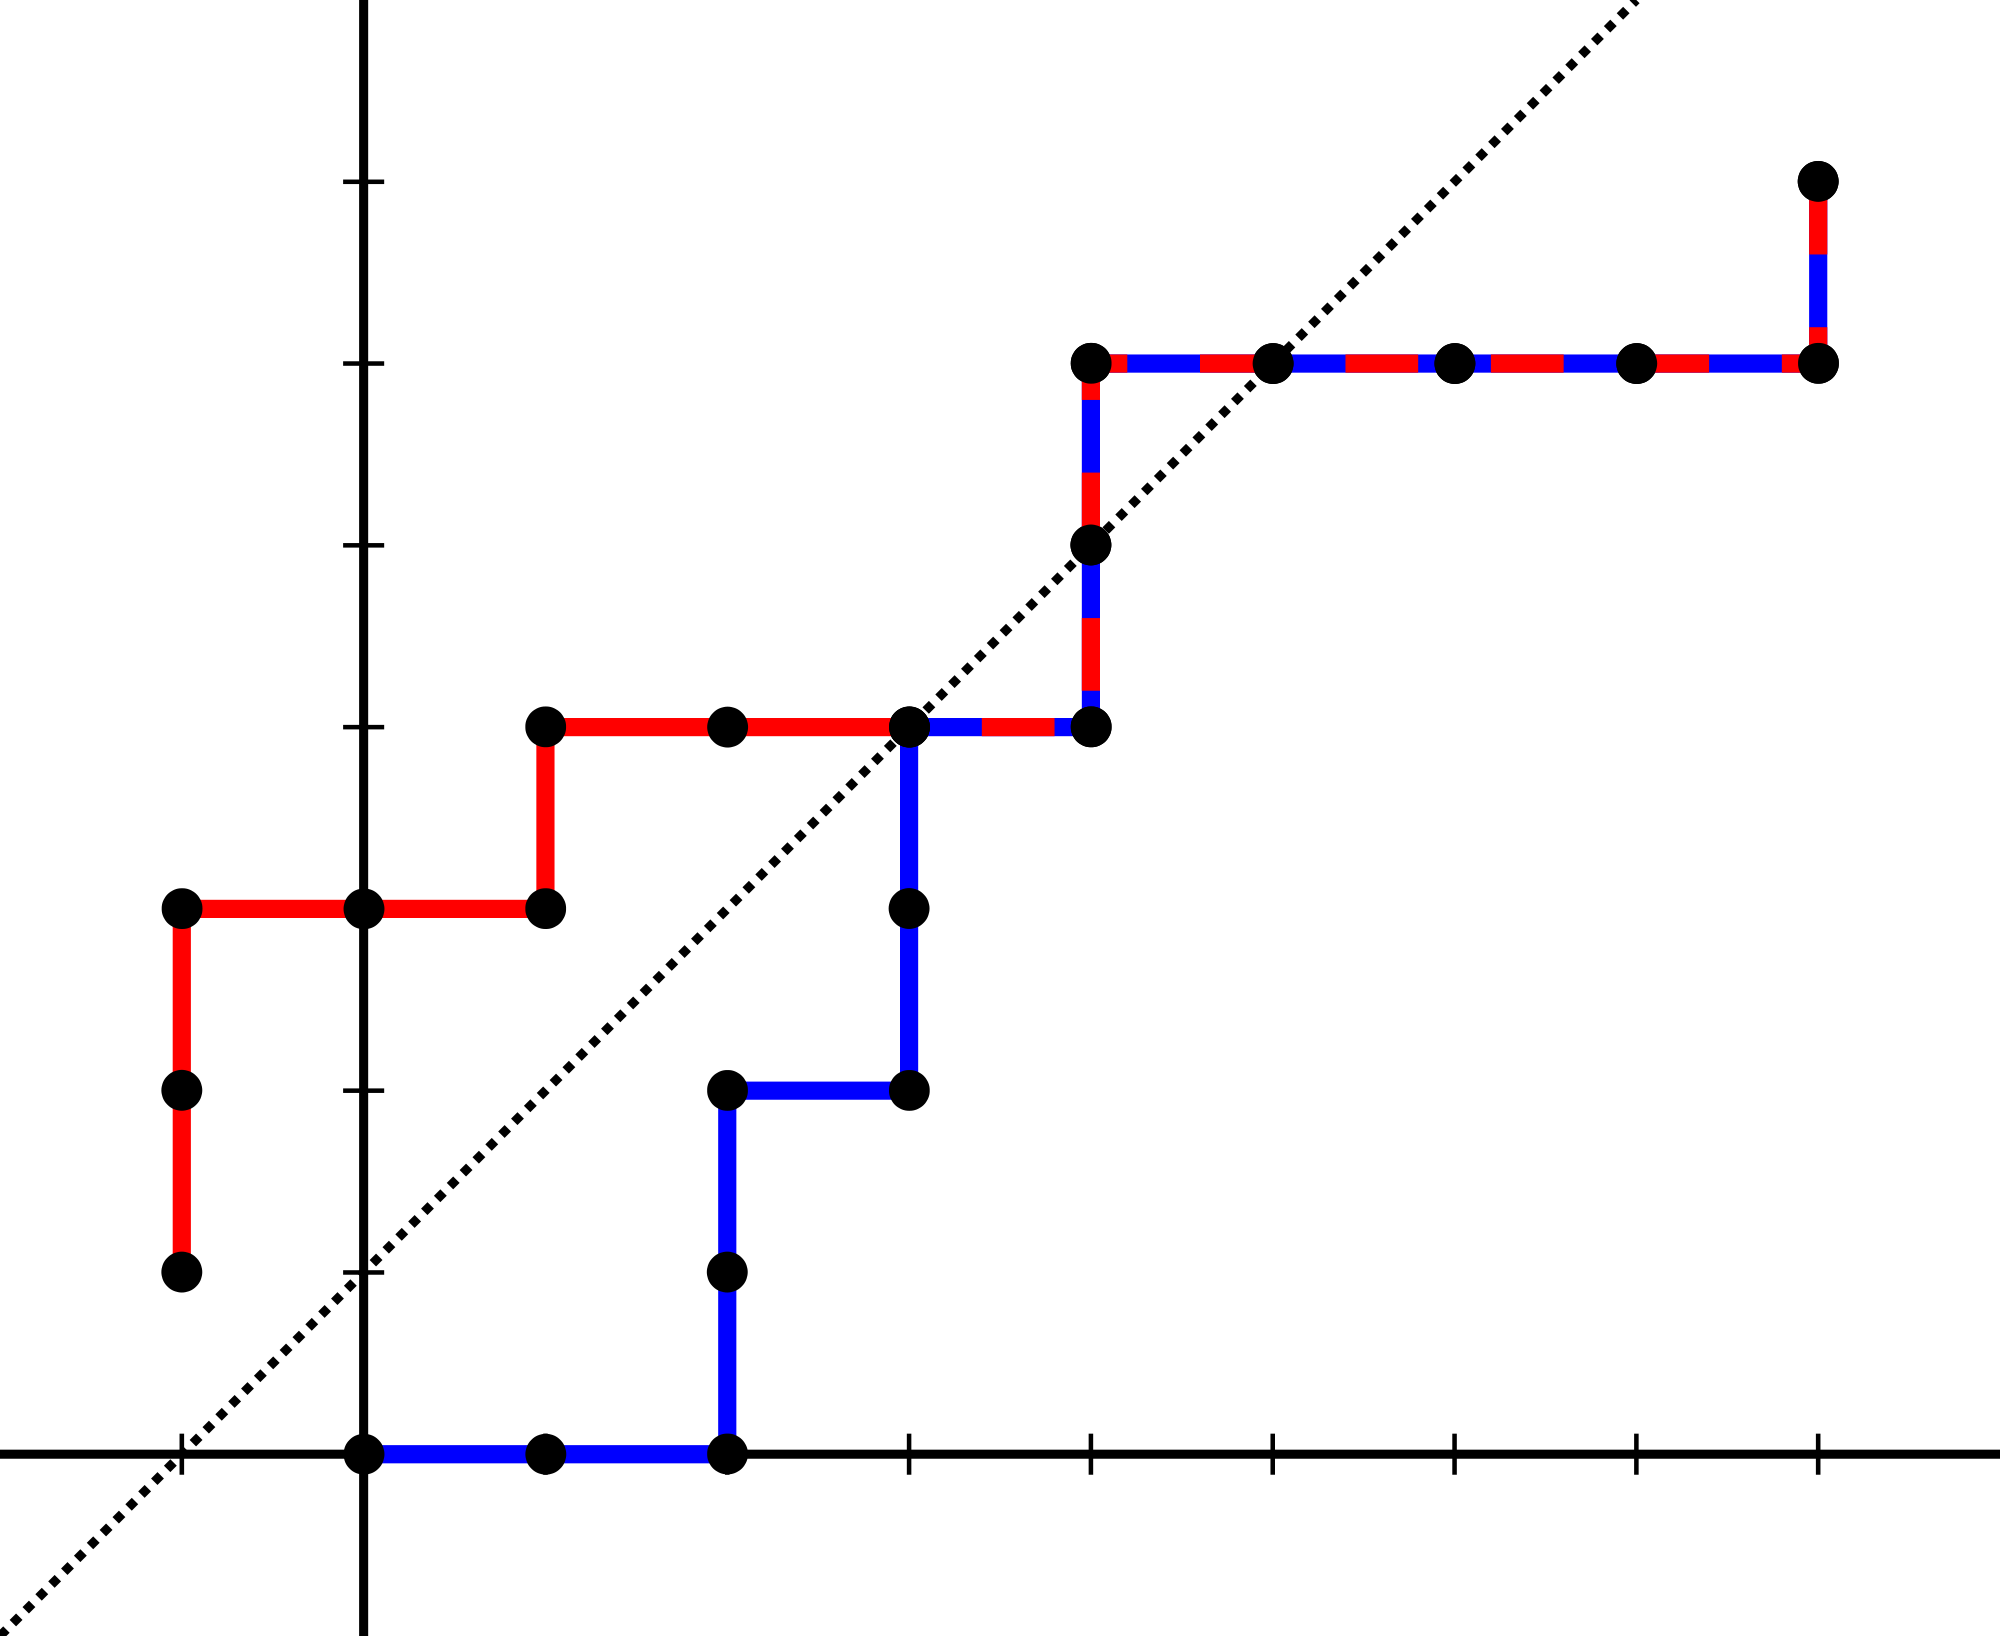
\includegraphics[width=150pt]{2000px-AndreReflection.png}
%	\caption{Bertrand's Ballot prob allowing Ties}
%	\label{fig:Bertrand's_Ballot_prob}
%\end{figure}

An interesting application of this is the famous Catalan number formula, which can be introduced under the random walk story. A random walk on the integers is to take $n$ steps of unit length, beginning at the origin and ending at the point $m$, that never become negative. Assuming $n$ and $m$ have the same parity and $n \ge m \ge 0$, this number is, according to the Bertrand's Ballot prob allowing ties,
\begin{equation*}
	{n \choose \frac{n+m}{2}} - {n \choose \frac{n+m}{2}+1} = \frac{m+1}{\frac{n+m}{2}+1} {n \choose \frac{n+m}{2}}
\end{equation*}
Here, $p+q=n$ and $p-q=m$, compared to our used settings. When $m=0$ and $n$ is even, this gives the Catalan number $\frac{1}{\frac{n}{2}+1} {n \choose \frac{n}{2}}$.

Let's tweak this prob a little bit more. Let's say candidate A starts at $a$ ``bonus'' votes, not 0. That is to say, the system goes from $(0,a)$ to $(p+q,p+a-q)$. If we do not allow ties, all paths hit the x-axis will be unfavorable, and the number of these paths equals the number of paths from $(0,a)$ to its ``mirror'' point $(p+q,-p-a+q)$. So, there are in total ${p+q \choose p+a}$ unfavorable paths, and the probability is $1 - \frac{{p+q \choose p+a}}{{p+q \choose p}}$. Note when $a=0$, there is already a tie, and the question really should be asked as: ``What if the first count is A, and then the process never has a tie''. So the probability should compute as:
\begin{equation*}
	1 - \frac{p}{p+q} \frac{{p-1+q \choose p-1}}{{p-1+q \choose p-1}} = \frac{p-q}{p+q}
\end{equation*}
It should have no prob with $a>0$.

If we allow ties, the ``mirror'' point should be reflected against $y=-1$, so it becomes $(p+q,-2-p-a+q)$. Now, suppose we go up $u$ steps and go down $d$ steps. Solving the following equations:
\begin{eqnarray*}
	u+d & = & p+q\\
	u+a-d & = & -2-p-a+q
\end{eqnarray*}
gives us $u=q-a-1$ and $d=p+a+1$. So there are ${p+q \choose p+a+1}$ paths unfavorable, and the probability is then $1-\frac{{p+q \choose p+a+1}}{{p+q \choose p}}$. When $a=0$, this becomes $\frac{p+1-q}{p+1}$, which agrees with what we obtained earlier.

In summary, if one starts at $(0,a)$ and ends at $(p+q,p+a-q)$, the number of unfavorable paths is $p+q \choose p+a$ if not allowing ties, $p+q \choose p+a+1$ if allowing ties.


\section{Catalan Number}
In chapter \ref{chapter: Bertrand_Ballot_prob}, we first met Catalan number from the generalized Bertrand's Ballot prob. We write here again the definition of Catalan number, with an intuitive interpretation.

The Catalan number is defined as,
\begin{equation}
	C_n = \frac{1}{n+1} {2n \choose n}
\end{equation}
The underlying story reads: Given two urns, one with $n$ red balls and the other with $n$ black balls, we want to draw one ball at a time (either red or black), such that at no time the number of pre-specified color is less than its alternative.

Since the Catalan number is associated with two equal-sized sets, it is oftentimes co-occurrent  with the words "pair", "full binary", and etc. 
\section{Conditional Probability}
\begin{deff}
	If $P(F) > 0$, then
	\begin{equation}
		P(E|F) = \frac{P(E,F)}{P(F)}
	\end{equation}
	$P(E|F)$ is called the conditional probability of $E$ given $F$. Conditional probability agrees with Definition \ref{def:probability}, and should be treated in the same way.
\end{deff}

\begin{deff}
	The multiplication rule
	\begin{equation}
		P(E_1, E_2, \ldots, E_n) = P(E_1) P(E_2|E_1) \ldots P(E_n|E_1, \ldots, E_{n-1})
	\end{equation}
\end{deff}

\begin{deff}
	Bayes' Formula
	\begin{equation}
		P(A_i|B) = \frac{P(B|A_i)P(A_i)}{P(B)}
	\end{equation}
	where $P(A_i)$ is sometimes called the prior distribution, $P(B|A_i)$ the likelihood function, and $P(A_i|B)$ the posterior distribution. The partition function $P(B)$ can be computed using the law of total probability
	\begin{equation}
		P(B) = \sum^n_{j=1}P(B|A_j)P(A_j)
	\end{equation}
\end{deff}

\begin{deff}
	Two events $E$ and $F$ are said to be {\em{independent}} if	
	\begin{equation}
		P(E,F) = P(E)P(F)
	\end{equation}
	A set of events are independent if every finite subset of these events is independent.
\end{deff}

\section{Conditional Probability}
\section{Conditional Expectation}
\section{Conditional Independence} 
\section{Probaility Space}
\section{Sample Space, Events, and Probability}
\begin{deff}
	A sample space $S$ is a set of all possible outcomes of an experiment. An outcome is also called a sample point.
\end{deff}
Note, when an experiment consists of several repetitions, each one of them is called a {\em{trial}}. As an example, if one decides to toss a coin 42 times, we can call each toss a trial of the experiment composed of 42 ones.

\begin{deff}
	An event $E$ is a subset of the sample space $S$. If the outcome of the experiment is contained in $E$, then we say that $E$ occurred.
\end{deff}

\begin{deff}\label{def:probability}
In short, a probability space is a measure space such that the measure of the whole space is equal to one. The expanded definition is following: a probability space is a triple $(\Omega,\; \mathcal{F},\; P)$ consisting of:
\begin{itemize}
\item the sample space $\Omega$ --- an arbitrary non-empty set,
\item the $\sigma-algebra$ $\FF \in 2^\Omega$ (also called $\sigma-filed$) --- a set of subsets of $\Omega$, called events, such that:
	\begin{itemize}
	\item $\FF$ contains the empty set: $\emptyset \in \FF$,
	\item $\FF$ is closed under complements: if $A \in \FF$, then also $(\Omega \setminus A) \in \FF$,
	\item $\FF$ is closed under countable unions: if $A_i \in \FF$ for $i=1,2,\ldots$, then also ($\bigcup A_i) \in \FF$,
	\end{itemize}
\item the probability measure $P: \FF \rightarrow [0,1]$ --- a function on $\FF$ such that:
\item $P$ is countably additive: if $\{A_i\} \in \FF$ is a countable collection of pairwise disjoint sets, then $P(\bigcup A_i) = \sum P(A_i)$, where $\bigcup$ denotes the disjoint union,
\item the measure of entire sample space is equal to one: $P(\Omega)=1$.
\end{itemize}
\end{deff}

\section{Probability Axioms}
\subsection{Law of Total Probability}
Suppose $B_n (n=1,2,3,\cdots$ is a finite or countably infinity partition of the sample space, then for an event $A$
\begin{align}
	Pr(A) = \sum_n Pr(A,B_n)
\end{align}
or,
\begin{align}\label{eq:Law of Total Probability}
	Pr(A) = \sum_n Pr(A|B_n) Pr(B_n)
\end{align}
It can also be stated for conditional probabilities. Suppose $X$ is an event in the same sample space, we have
\begin{align}
	Pr(A|X) = \sum_n Pr(A|B_n,X)Pr(B_n|X)
\end{align}
One application of Eq~\ref{eq:Law of Total Probability} is when calculating $Pr(A)$ is difficult, we can introduce an ``auxiliary variable'' $B$, in the hope that the conditional probability $Pr(A|B_n)$ is easier to compute.
\subsection{Law of Total Variance}
\subsection{Law of Total Covariance}
\subsection{Law of Total Expectation}
\subsection{Law of Total Cumulance}
\subsection{Probability Inequalities}

\section{Types of Probabilities: Frequentism and Bayesian} 
\section{Random Variables}
The Laplace distribution can be written as an infinite mixture of Gaussians with variance $w$ distribution according to an exponential distribution. An exponential distribution can be written as a $\chi^2$ distribution with two degrees of freedom.
\section{Continuous Random Variables}
\section{Discrete Random Variables}
\section{Joint Distributed Random Variables}
\section{Random Vectors/Matrices}
\section{Function of Random Variables}
\subsection{Transformation}
\subsection{Convolutions: Sum of Normally Distributed Random Variables}
\subsection{Product Distribution}
\subsection{Ratio Distribution} 
\chapter{Useful Distributions}
\section{Discrete Distributions}
\subsection{Poisson Distribution}
\subsection{Bernoulli Distribution}
\subsection{Binomial Distribution}
\subsection{Negative Binomial Distribution}
\subsection{Categorical Distribution}
\subsection{Multinomial Distribution}
\subsection{Geometric Distribution}
\subsection{Hyper-Geometric Distribution}
\subsection{Poisson Distribution}
\section{Continuous Distributions}
\subsection{Uniform Distribution}
\subsection{Exponential Distribution}
\subsection{$\chi^2$ Distribution}

\subsection{Gaussian Distribution}
\subsubsection{Univariate Gaussian}
\subsubsection{Multivariate Gaussian}
\begin{align}
	f(\x|\bmu,\bSigma) = \frac{1}{\sqrt{2\pi|\bSigma|}} \exp\left\{-\frac{1}{2}(\x-\bmu)^T\bSigma^{-1}(\x-\bmu)\right\}
\end{align}
Using the technique of `completing the square', we have
\begin{align}
	f(\x_1|\x_2) &= \frac{f(\x_1,\x_2)}{f(\x_2)}\\
	&= \frac{1/\sqrt{2\pi|\bSigma|}\exp\left\{-\frac{1}{2}(\x-\bmu)^T\bSigma^{-1}(\x-\bmu)\right\}}{1/\sqrt{2\pi|\bSigma_{22}|}\exp\left\{-\frac{1}{2}(\x_2-\bmu)^T\bSigma_{22}^{-1}(\x_2-\bmu)\right\}}\\
	&= C \cdot \exp\left\{-\frac{1}{2}(\x-\bmu)^T\bSigma^{-1}(\x-\bmu)\right\}\\
	&= C \cdot \exp\left\{-\frac{1}{2}[(\x_1-\bmu_1)^T\bLambda_{11}(\x_1-\bmu_1)+(\x_1-\bmu_1)^T\bLambda_{12}(\x_2-\bmu_2)+(\x_2-\bmu_2)^T\bLambda_{21}(\x_1-\bmu_1)]\right\}\\
	&= C \cdot \exp\left\{-\frac{1}{2}\x_1^T\bLambda_{11}\x_1 + \x_1^T[\bLambda_{11}\bmu_1 - \bLambda_{12}(\x_2-\bmu_2)]\right\}	
\end{align}
Hence
\begin{align}
	\bSigma_{1|2} &= \bLambda_{11}^{-1}\\
	\bmu_{1|2} &= \bmu_1 - \bLambda_{11}^{-1}\bLambda_{12}(\x_2-\bmu_2)
\end{align}
or
\begin{align}
	\bSigma_{1|2} &= \bSigma_{11} - \bSigma_{12}\bSigma_{22}^{-1}\bSigma_{21}\\
	\bmu_{1|2} &= \bmu_1 + \bSigma_{12}\bSigma_{22}^{-1}(\x_2-\bmu_2)
\end{align}

\subsection{Dirichlet Distribution}
\subsubsection{Gamma Function and Beta Function}
The {\em{gamma function}} is defined for all complex numbers except the non-positive integers. For complex numbers with a positive real part, it is defined via an improper integral that converges:
\begin{equation}
	\Gamma(z) = \int_0^\infty e^{-t} t^{z-1} dt
\end{equation}
For all positive numbers $z$,
\begin{equation}
	\Gamma(z) = (z-1)\Gamma(z-1)
\end{equation}
and in particular, if $n$ is a positive integer:
\begin{equation}
	\Gamma(n) = (n-1)!
\end{equation}
Note, the gamma function shifts the normal definition of factorial by 1.

The {\em{beta function}} is defined by
\begin{equation}
	B(x,y) = \int_0^1 t^{x-1} (1-t)^{y-1} dt
\end{equation}
for $Re(x), Re(y) > 0$.

It can also be written as
\begin{equation}
	B(x,y) = \frac{\Gamma(x) \Gamma(y)}{\Gamma(x+y)}
\end{equation}

\subsubsection{Introduction}
The Dirichlet distribution of order $K \ge 2$ with parameters $\alpha_1, \dots, \alpha_K > 0$ has a probability density function with respect to Lebesgue measure on the Euclidean space $\RR^{K-1}$ given by
\begin{equation}
	f(x_1, \dots, x_{K-1}; \alpha_1, \dots, \alpha_K) = \frac{1}{B(\balpha)} \prod^K_{i=1} x_i^{\alpha_i-1}
\end{equation}
for all $x_1, \dots, x_K > 0$ and $x_1 + \dots + x_K = 1$. The density is zero outside this open\footnote{``Open'' here means none of the $x_i$'s can be 1, actually $x_i \in (0,1)$.} $(K-1)$-dimensional simplex.

The normalizing constant is the multinomial beta function, which can be expressed in terms of the gamma function:
\begin{equation}
	B(\balpha) = \frac{\prod_{i=1}^K \Gamma(\alpha_i)}{\Gamma(\sum_{i=1}^K \alpha_i)}, \mbox{ where } \balpha=(\alpha_1, \dots, \alpha_K)
\end{equation}


\subsection{$t$ Distribution}
\subsection{Inverse Gaussian Distribution}
\subsection{log-normal Distribution}
\subsection{Laplace Distribution}
\subsection{Beta Distribution}
\subsection{Gamma Distribution}
\subsection{Wishart Distribution}
\section{Quantitative Measure and Characteristic Functions}
\section{Describing Shape of a Distribution: Skewness, Kurtosis}
\section{Describing a Sample: Mean, Variance}
\section{Degrees of Freedom, Mean, Variance, and Moment, Central Moment, Cumulant, Law of the unconscious statistician}
\section{Percentile and Median}
\section{Coefficient of Variation}
\section{Covariance and Correlation}
\section{Moment Generating Function}
\section{Characteristic Function}

\section{Limit Theorems}
\section{Markov and Chebyshev Inequalities}
\begin{thm}
	{\underline{Markov's Inequality}}. If $X$ is a random variable that takes only nonnegative values, then for any value $a > 0$, $$P\{X \ge a\} \le \frac{E[X]}{a}$$
\end{thm}

\begin{thm}
	{\underline{Chebyshev's Inequality}}. If $X$ is a random variable with finite mean $\mu$ and variance $\sigma^2$, then, for any value $k > 0$, $$P\{|X-\mu| \ge k\} \le \frac{\sigma^2}{k^2}$$
\end{thm}

\section{Weak Law of Large Numbers}
\begin{thm}
	{\underline{The Weak Law of Large Numbers}}. Let $X_1, X_2, \cdots$ be a sequence of i.i.d. random variables, each having finite mean $E[X_i] = \mu$. Then, for any $\epsilon > 0$, $$P\left\{\left|\frac{X_1+\cdots+X_n}{n} - \mu\right| \ge \epsilon \right\} \to 0 \mbox{ as } n \to \infty$$
\end{thm}

\section{Central Limit theorem}
\begin{thm}
	{\underline{Central Limit theorem}}. Let $X_1, X_2, \cdots$ be a sequence of independent and identically distributed random variables, each having mean $\mu$ and variance $\sigma^2$. Then the distribution of $$\frac{\frac{X_1+\cdots+X_n}{n}-\mu}{\sqrt{\sigma^2/n}} = \frac{X_1+\cdots+X_n - n\mu}{\sigma \sqrt{n}}$$ tends to the standard normal as $n \to \infty$.
\end{thm} 
\section{Selected Topics of Probability}
\section{Indicator Variables}
\section{Ordered Statistics}
\section{Copula}
\section{coupling}
\section{The Reflection Principle}



\section{Elementary Theory of Stochastic Processes}
%!TEX root = ../Probability.tex

\chapter{Introduction}
\deff{
	A \emph{stochastic process} is a collection of random variables $X(t)$ for $t \in T$, where the \emph{time} parameter $T$ is usually\footnote{It can be defined in a general space.} a subset of $\RR$. The set $\mathscr{S}$ containing all possible values of $X(t)$ is called the \emph{state space} of the process.
}

There are four common types of stochastic processes (with corresponding examples):
\begin{table}[h]
\centering
  \begin{tabular}{ | c | c | c | }
    \hline
     & \textbf{Finite or Countable State Space} & \textbf{Continuous State Space} \\ \hline
    \textbf{Discrete Time} & Markov Chains & Harris Chains \\ \hline
    \textbf{Continuous Time} & Poisson Processes and Hawkes Processes & Gaussian Processes and Wiener Processes \\ \hline    
  \end{tabular}
  \small{\caption{Four Common Types of Stochastic Processes.}}
\end{table}

\deff{
	A {\em{renewal process}} is an idealized stochastic model for events that occur randomly in time (generically called renewals or arrivals). The basic mathematical assumption is that the times between the successive arrivals are independent and identically distributed (i.i.d.). 
}

\deff{
	A {\em{delayed renewal process}} is just like an ordinary renewal process, except that the first arrival time is allowed to have a different distribution than the other inter-arrival times.
}


\deff{
	A {\em{counting process}} is a stochastic process $\{N(t), t \ge 0\}$ with values that are non-negative, integer, and increasing:
}

\deff{
	A {\em{point process}} is a collection of mathematical points randomly located on some underlying mathematical space such as the real line, the Cartesian plane, or more abstract spaces.
}

\deff{
	A {\em{diffusion process}} is a solution to a stochastic differential equation. For example, Brownian motion.
}

\deff{
	A {\em{jump process}} is a type of stochastic process that has discrete movements, called jumps, with random arrival times, rather than continuous movement, typically modeled as a simple or compound Poisson process.
}
\chapter{Markov Chains}
\section{Introduction}
\deff{
The \emph{Markov property} is defined by the requirement that
\begin{align}
	P(X_{n+1}=x_{n+1} \vert X_0=x_0,\cdots,X_n=x_n) = P(X_{n+1}=x_{n+1} \vert X_n=x_n)
\end{align}
}
\deff{
	The conditional probabilities $P(X_{n+1}=y \vert X_n=x)$ are called the \emph{transition probabilities} of the chain.
}

\deff{
	We say a Markov chain has \emph{stationary transition probabilities} if the transition probabilities $P(X_{n+1}=y \vert X_n=x)$ is independent of the time $n$.
}

From now on, when we say that $X_n, n \ge 0$ forms a Markov chain, we mean that these random variables satisfy the Markov property and have stationary transition probabilities.

\deff{
	A state $a$ of a Markov chain is called an \emph{absorbing state} if $P(a,a) = 1$ or, equivalently, if $P(a,y) = 0$ for all $y \ne a$.
}

\section{Discrete Time Markov Chains}
\subsection{Gambler's Ruin}
\subsection{Discrete Time Branching Processes}

\section{Continuous Time Markov Chains}

\section{Poisson Processes}
\section{Poisson Processes on the Line}
\section{Variable Rate Poisson Processes}
\section{Poisson Processes in Higher Dimensions} 
\chapter{Renewal Theory}   
\section{Renewal theory for positive lattice valued random variables as connected with Markov chains: Blackwell's renewal theorem for positive lattice valued random variables}
\section{Selected Topics of Stochastic Processes}
\section{Martingales which are functions of discrete time Markov chains}
\section{Brownian motion: Path properties, reflection principle, random walk approximation.}
\section{Random Fields}
\section{Discrete and Continuous Time Birth and Death processes}
\section{Discrete and Continuous Time Queuing processes}
\section{Finite State Space Pure Jump Processes}
\section{Infinite Server Queue}


\section{Measure-theoretical Probability}
\section{Why Do We Need Rigorous Probability Theory?}
Let's recall the axioms from non-measure probability courses. We have a \emph{sample space} $\Omega$, the elements of which $w \in \Omega$ called \emph{outcomes}, and the subsets $E \subset \Omega$ called \emph{events}. \emph{Probability measure} is nothing but assigning probability $P(E)$ to each event $E \subset \Omega$, under the following constraints:
\begin{enumerate}
	\item $P(E) \in [0,1]$
	\item $P(\Omega) = 1$
	\item $P(\uplus_{i=1}^\infty E_i) = \sum_{i=1}^n P(E_i)$
\end{enumerate}
where in the last constraint, `$\uplus$' means the union of \emph{disjoint} sets.

One of the motivations\footnote{Add unification of discrete and continuous r.v's.} of developing measure-theoretical probability theory is triggered by the following question:

\vspace{2 mm}
\textbf{Q: \emph{How do we know the three listed axioms are consistent, in particular, the last constraint?}}
\vspace{0.5 mm}

Actually, the \emph{Banach-Tarski paradox} and the \emph{Vitali paradox} are such counter examples (TBA). We have two choices: either we could reject the \emph{axiom of choice}, which is one of the basic assumptions made in the two paradoxes; or we could claim there are some subsets $E \subset \Omega$ that is `non-measurable'. In this course, we take the second solution.

\section{Normal Numbers}
\deff{
	Every $X \in [0,1]$ has a binary decimal expansion $X = 0.d_1d_2d_3\cdots$ or $X = \sum_{k=1}^\infty d_k 2^{-k}$, $d_k \in \{0,1\}$. However, it is possible that $X$ may have two expansions, for example, $X=0.111\cdots = 0.1000\cdots$. We choose the expansion ending in all 1's to make it well-defined.
}

\deff{
	$X \in (0,1)$ is normal if $\lim\limits_{n \to \infty} \frac{1}{n} \sum_{k=1}^n d_k = \frac{1}{2}$.
}

\prop{
	If $X \sim U(0,1)$, then $P(X\mbox{ is normal}) = 1$.
}

\lem{
	Suppose that $X_1, X_2, \cdots$ are i.i.d $Ber(1/2)$. Then $X = \sum_{n=1}^\infty X_n 2^{-n}$ is uniform on $(0,1)$.
}
\prof{	
	We (only) need to show $P(X \in (a,b]) = b - a$.\\
	
	Case 1: $\exists k, s.t. (a,b] = ((k-1)2^{-n}, k2^n]$. Since $(k-1)2^{-n} = 0.d_1d_2 \cdots d_n000\cdots$,
	\begin{align}
		P(X \in ((k-1)2^{-n},k2^{-n}]) &= P(X_1=d_1,X_2=d_2,\cdots,X_n=d_n, X_i=1 for i > n) = 2^{-n} = b-a
	\end{align}

	Case 2: $(a,b] = (l2^{-n},k2^{-n}], l < k$.
	\begin{align}
		P(X \in (l2^{-n},k2^{-n}]) &= (k-l)2^{-n} = b- a
	\end{align}

	In general, if $a < b$, let $a_n, b_n \in 2^{-n}\Z$ be s.t. $a_n \le a < a_n + 2^{-n}, b_n - 2^{-n} \le b < b_n$, then
	\begin{align}
		P(X \in (a,b]) \le P(X \in (a_n,b_n]) = b_n - a_n
	\end{align}
	$b_n - a_n - 2^{-n+1} = P(X \in (a_n+2^{-n},b_n-2^{-n}) \le \epsilon$. Note, $b-a \le b_n - a_n \le b- a + 2^{-n+1}$.

	We need to show that $P(\lim\limits_{n \to \infty} \frac{1}{n} \sum_{k=1}^\infty = \frac{1}{2}) = 1$. This is the SLLN.
}

We know that $\{X \in (a,b]\}$ are events. Why is $\{X\mbox{ is normal}\}$ an event?
\begin{align}
	\{X\mbox{ is normal}\} = \left\{\lim\limits_{n \to \infty} \frac{1}{n} \sum_{k=1}^\infty = \frac{1}{2}\right\} = \bigcap_{l=1}^\infty \bigcup_{m=l}^\infty \bigcap_{n=m}^\infty \left\{\left\vert \frac{1}{n} \sum_{k=1}^\infty - \frac{1}{2} \right\vert < \frac{1}{l} \right\}
\end{align}
This is equivalent to $\forall \epsilon = \frac{1}{l} > 0, \exists m < \infty, s.t., |\frac{1}{n} \sum_{k=1}^\infty - \frac{1}{2}| < \epsilon, \forall n \ge m$.

\section{Formal Definition of Probability Space}
\deff{
	A collection $\FF$ of subsets of $\Omega$ is a $\sigma$-field (or algebra) if
	\begin{enumerate}
		\item $\FF$ is non-empty;
		\item If $A \subset \FF$, then $A^c \in \FF$ (closed under complement);
		\item If $\{A_i\}$ is a countable sequence of elements of $\FF$, then $\cup_i A_i \in \FF$ (closed under countable unions).
	\end{enumerate}	
}
Note, 1) $\Omega \in \FF, \emptyset \in \FF$ since $\Omega = A \cup A^c if A \in \FF$. $\emptyset = \Omega^c$. 2) $\FF$ is closed under countable intersections.

\deff{
	A \emph{measure space} is a pair $(\Omega, \FF)$ where $\FF$ is a $\sigma$-field of subsets of $\Omega$.
}

\deff{
	A non-negative measure $\mu$ on $(\Omega, \FF)$ is a function $\mu: \FF \to \bar \RR_+ = [0,\infty]$ s.t.
	\begin{enumerate}
		\item $\mu(\emptyset) = 0$;
		\item If $A_i$ is a sequence of disjoint sets in $\FF$, then $\mu(\uplus_{i=1}^\infty A_i) = \sum_{i=1}^\infty \mu(A_i)$.
	\end{enumerate}
}

\deff{
	A \emph{probability space} is a triple $(\Omega, \FF, P)$ where $(\Omega, \FF)$ is a measure space, and $P$ is a measure on $(\Omega, \FF)$ with $P(\Omega) = 1$.
}

\ex{
	$\FF = 2^{\Omega}$ (all subsets of $\Omega$). If $\Omega = \Z$, then usually, $\FF = 2^\Omega$ is the $\sigma$-field we use. If $\Omega=(0,1]$ or $\R$, then $\FF$ is usually too big.
}

\ex{
	Let $\AA \subset 2^\Omega$, then $\sigma(\AA)$ is the smallest $\sigma$-field containing $\AA$. If $\OO \subset \R$ is the collection of all open subsets of $\R$, then $\sigma(\OO) = \BB$ is called the \emph{Borel $\sigma$-field}.
}

\section{Lecture 5 (1/21/2015 Wednesday): }
(Today and Friday) in Appendix A.
\deff{
	A non-empty collection of subsets $\AA \subset 2^\Omega$ is called an algebra if
	\begin{enumerate}
		\item $A \in \AA$ then $A^c \in \AA$
		\item $A, B \in \AA$ then $A \cup B \in \AA$
		\item $A, B \in \AA$ then $A \cap B \in \AA$
	\end{enumerate}
}

\deff{
	$\mu: \AA \rightarrow [0,\infty]$ is a measure on the algebra $\AA$ if
	\begin{enumerate}
		\item $\mu(\emptyset) = 0$
		\item If $\uplus_{i=1}^\infty A_i \in \AA$ then $\mu(\uplus_{i=1}^\infty A_i) = \sum_{i=1}^\infty \mu(A_i)$
	\end{enumerate}
}

\deff{
	A measure $\mu$ is $\sigma$-finite (on an algebra or a $\sigma$-field) if $\exists$ a sequence $A_n \nearrow \Omega$ with $\mu(A_n) < \infty$ ($A_n \subset A_{n+1}$ and $\Omega = \cup_{i=1}^\infty A_n$)
}

\begin{thm}
	(Caratheodory Extension) Let $\mu$ be a $\sigma$-finite measure on an algebra $\AA$. Then $\mu$ has a unique extension to a measure on $(\Omega, \sigma(\AA))$.
\end{thm}

Note: Meausre on algebras also satisfy Themorem 1.1.1
\begin{enumerate}
	\item $A \subset B$ then $\mu(A) \le \mu(B)$
	\item $\mu(\cup_{i=1}^\infty A_i \le \sum_i \mu(A_i)$ if $\cup A_i \in \AA$
\end{enumerate}


\section{Probability Space and Measure}

\section{Algebra of Sets}

\subsubsection{Set Operations}
Given two sets $A, B \in \Omega$, there are four basic binary operations on sets:
\begin{enumerate}
	\item {\em{Union}}: $A \cup B = \{x: x \in A \mbox{ or } x \in B\}$
	\item {\em{Intersection}}: $A \cap B = \{x: x \in A \mbox{ and } x \in B\}$
	\item {\em{Set difference}}: $A \setminus B = \{x: x \in A \mbox{ and } x \notin B\}$
	\item {\em{Set complement}}: $A^c = \Omega \setminus A$
\end{enumerate}

Set complement is the ``strongest'' operation, because if a collection of sets $\AA$ is closed under complement, and if it is also closed under any one of the other three operations, $\AA$ is closed under the rest two. That is seen from,
\begin{align}
	\mbox{If closed under } union &
	\begin{cases}
		A \cap B = (A^c \cup B^c)^c\\
		A \setminus B = A \cap B^c = (A^c \cup B)^c
	\end{cases}	
	\\
	\mbox{If closed under } intersection &
	\begin{cases}
		A \cup B = (A^c \cap B^c)^c\\		
		A \setminus B = A \cap B^c
	\end{cases}
	\\
	\mbox{If closed under } difference &
	\begin{cases}
		A \cap B = A \setminus (A \setminus B)\\
		A \cup B = (A^c \cap B^c)^c = (A^c \setminus (A^c \setminus B^c))^c\\
	\end{cases}		
\end{align}

The difference operation is the second ``strongest'' operation, in that if a collection of sets $\AA$ is closed under difference, it is closed under intersection, that is seen from,
\begin{align}
	A \cap B = A \setminus (A \setminus B)
\end{align}

The third ``strongest'' operation is the union, which can not be implied from difference or intersection, or their combination.

The ``weakest'' operation is the intersection, which can be implied from the difference.

%To summarize, the ``strongest'' pair would be the complement plus any one more, which implies everything else; the second ``strongest'' would be the difference plus the union, which implies the intersection but not the complement ($\Omega$ may not be in the collection). \smallmarginpar{\textdbend}

\subsubsection{Class of Set Collection}
\begin{deff}
	Given a set $\Omega$, a non-empty collection $\PP \subset 2^\Omega$ is called a {\em{$\pi$-system}} iff:
	
	\center{$\forall A, B \in \PP$, $A \cap B \in \PP$}
\end{deff}
Notice, this has the weakest requirement.

\begin{deff}
	Given a set $\Omega$, a non-empty collection $\QQ \subset 2^\Omega$ is called a {\em{semiring}} iff:
	
	\center{$\forall A, B \in \QQ \mbox{ and } A \supset B$}
	\center{$\exists C_k \subset \QQ, s.t., A \setminus B = \bigcup_{k=1}^n C_k$}
\end{deff}

\begin{deff}
	Given a set $\Omega$, a non-empty collection $\RR \subset 2^\Omega$ is called a {\em{ring}} iff:
	
	\center{$\forall A, B \in \RR$, $A \cup B \in \RR$ and $B \setminus A \in \RR$}
\end{deff}

There are two points need to mention: the empty set is in a ring, since $A \setminus A = \emptyset$; $\AA$ is also closed under intersection (the reverse need not be true).

\begin{deff}
	A {\em{ring}} $\AA$ is called an {\em{field}} iff $\Omega \in \AA$.
\end{deff}
So a field is closed under all {\em{finite}} combination of set operations.


\begin{deff}
	An {\em{field}} is called a {\em{$\sigma$-field}} if for any sequence ${A_n}$ of sets in $\AA$, $\cup_{n \ge 1} A_n \in \AA$.
\end{deff}

$\not \exists$

\section{Integration Theory}
\section{Random Variables}
\section{Law of Large Numbers}
\section{Types of Convergence}
\subsubsection{Convergence in Distribution}
\subsubsection{Convergence in Probability}
\subsubsection{Almost Surely Convergence}
\subsubsection{$L^p$ Convergence}

\section{Weak Law of Large Numbers (WLLN)}
\section{Strong Law of Large Numbers (SLLN)}

\section{Central Limit theorem}

\section{Some Tricks}
\section{Prove by Contraposition}

\section{Construct Finer Partition}
Given twofinite partitions $\{A_n\}$ and $\{B_m\}$, a finer partition can be constructed as
\begin{align*}
	(\cup_{i=1}^n A_i) \bigcap (\cup_{j=1}^m B_j) = \bigcup (\cap_{i=1}^n \cap_{j=1}^m A_i B_j)
\end{align*}

\section{Prove Equality}
To prove two numerical quantities are equal $X=Y$, often times we can do this by showing $X \le Y$ and $X \ge Y$. Similarly, to prove two sets are equal $E = F$, we can show $E \subset F$ and $E \subset F$.

\section{An Epsilon of Room}
If one has to show that $X \le Y$, try proving that $X \le Y + \epsilon, \forall \epsilon > 0$. This trick combines well with the ``Prove Equality'' trick.

In a similar spirit, if one needs to show that a quantity $X$ vanishes, try showing that $|X| \le \epsilon, \forall \epsilon > 0$.

If one wants to show that a sequence $x_n$ of real numbers converges to zero, try showing that $\limsup_{n \to \infty} |x_n| \le \epsilon, \forall \epsilon > 0$

%{\textbf{One caveat:}} for finite $x$, and any $\epsilon > 0$, it is true that $x + \epsilon > x$ and $x - \epsilon < x$, but it is not true when $x$ is equal to $+\infty$ or $-\infty$. \smallmarginpar{\textdbend}


\section{Interpretations of Probability}
\subsection{Cox's theorem}
\subsection{Principle of Maximum Entropy}

\section{Measure-theoretical Stochastic Processes}








\documentclass{book}
\usepackage{amssymb,amsmath,mathtools}


\usepackage{algorithm2e,algorithmic}

\usepackage{mathrsfs}
\usepackage{paralist}

\usepackage{esint} % for \fint

\allowdisplaybreaks

\usepackage{color}		% enable color characters
\usepackage{graphicx} 	% insert image files
\usepackage{enumerate} 	% enumerate items
\usepackage{caption}
\usepackage{subcaption}
\usepackage{multirow,multicol}
\usepackage[makeroom]{cancel}

\usepackage[colorlinks=true,linkcolor=blue,citecolor=blue]{hyperref}

\usepackage{makeidx}

\newcommand{\cem}[1]{\color{magenta}{\em{#1}}} % color emphasize
\newcommand{\dual}[2]{{#1}^{(#2)}} % color emphasize

\newcommand{\tr}{{\mathrm{tr}}}
\renewcommand{\vec}{{\mathrm{vec}}}

\newcommand{\dd}{{\,\mathrm{d}\,}}
%%
%% horizontal and vertical centering in table p mode
%%
\usepackage{array}
\newcolumntype{P}[1]{>{\centering\arraybackslash}p{#1}} % horizontal centering
\newcolumntype{M}[1]{>{\centering\arraybackslash}m{#1}} % vertical centering

%%
%% define bold font for the alphabet
%%
\usepackage{pgffor}
\foreach \letter in {a,...,z}{ % bold font for a..z
\expandafter\xdef\csname \letter \endcsname{\noexpand\ensuremath{\noexpand\mathbf{\letter}}}
}
\foreach \letter in {A,...,Z}{ % bold font for A..Z
\expandafter\xdef\csname \letter \endcsname{\noexpand\ensuremath{\noexpand\mathbf{\letter}}}
}
\foreach \letter in {A,...,Z}{ % `field' font for AA..ZZ
\expandafter\xdef\csname \letter\letter \endcsname{\noexpand\ensuremath{\noexpand\mathcal{\letter}}}
}
\foreach \letter in {A,...,Z}{ % `field' font for AAA..ZZZ
\expandafter\xdef\csname \letter\letter\letter \endcsname{\noexpand\ensuremath{\noexpand\mathbb{\letter}}}
}
\newcommand{\balpha}{{\boldsymbol{\alpha}}}
\newcommand{\bbeta}{{\boldsymbol{\beta}}}
\newcommand{\bgamma}{{\boldsymbol{\gamma}}}
\newcommand{\bkappa}{{\boldsymbol{\kappa}}}
\newcommand{\bmu}{{\boldsymbol{\mu}}}
\newcommand{\btheta}{{\boldsymbol{\theta}}}
\newcommand{\bTheta}{{\boldsymbol{\Theta}}}
\newcommand{\bPi}{{\boldsymbol{\Pi}}}
\newcommand{\bSigma}{{\boldsymbol{\Sigma}}}
\newcommand{\bPhi}{{\boldsymbol{\Phi}}}
\newcommand{\bLambda}{{\boldsymbol{\Lambda}}}
\newcommand{\bdeta}{{\boldsymbol{\eta}}}
\newcommand{\bphi}{{\boldsymbol{\phi}}}



%%
%% add definitions and theorems
%%
\usepackage[thmmarks,amsmath]{ntheorem}
\theorembodyfont{\normalfont}
\newtheorem{deff}{Definition}[section]
\newtheorem{thm}{Theorem}[section]
\newtheorem{prop}{Proposition}[section]
\newtheorem{lem}{Lemma}[section]
\newtheorem{cor}{Corollary}[section]
\newtheorem{rmk}{Remark}[section]
\newtheorem{alg}{Algorithm}[section]
\newtheorem{ex}{Example}[section]
\newtheorem{ques}{Question}[section]
\newtheorem{ans}{Answer}[section]
\newtheorem{prob}{Problem}[section]
\newtheorem{sol}{Solution}[section]
\newtheorem*{prof}{Proof}[section] 

\begin{document}
\title{Machine Learning}
\author{Xi Tan (xtan3.1415926@gmail.com)}

\maketitle
\tableofcontents
\chapter*{Preface}
This book project, which consists of four subjects: Finance, Mathematics, Statistics, and Computer Science, is tailored specifically to prepare someone for a quant career. It originated from my general belief of the hierarchy of solving a problem --- problems are solved at strategic, tactical, and operational levels.

{\em{Microeconomics}} and {\em{Macroeconomics}} explain the driving forces of capital markets, from a legislator's perspective. {\em{Accounting}} and {\em{Corporate Finance}} take a closer and necessary look at these forces, from a different angle. {\em{Stochastic Calculus}} and {\em{Asset Pricing}} provide with a set of tools and ideas that enables us to {\bf{strategically}} model one of the central problems in Quantitative Finance.

Generally speaking, there are two paths to solve a quantitative finance problem at the {\bf{tactical}} level: the mathematical way and the statistical way. There are only two pieces of math we need to know: {\em{Analysis}}, in particular measure-theoretical probability and differential equations; and {\em{Linear Algebra}}, with functional analysis in mind. Statistics, on the other hand, should start with {\em{Statistical Experiment Design}}, from which we learn how to collect data for statistical models. Next, the study of {\em{Random Variables}} and {\em{Stochastic Processes}} introduce the building blocks of the statistical ``pillbox'', with {\em{Mathematical Statistics}} the ``scaffold''. Once the ``pillbox'' is ready, we are equipped to tackle our problems using {\em{Machine Learning}}, which is essentially a collection of statistical models and optimization algorithms.

{\em{Computer Architecture}} and {\em{Operating System}} are respectively about the ``hardware'' and ``software'' of a single computer. The interaction of multiple computers is understood in {\em{Computer Network}}. Once we are comfortable with these concepts, we will be able to use {\em{Data Structure and Algorithms}} to solve problems at the {\bf{operational}} level, and use {\em{C++}} and/or {\em{Java}} to implement our ideas.

I am aware that it can take a while, and even multiple advanced degrees, to finish this curriculum, but let's remember the motto from the Leipzig Gewandhaus Orchestra: ``{\bf{\em{Res severa est verum gaudium}}}''.

\vspace{8mm}
\hfill {\em{Xi Tan}}

\hfill {\em{West Lafayette, IN}}

\hfill {\em{October, 2013}}

\addcontentsline{toc}{chapter}{Preface}


\chapter{Introduction}
There are two main types of Machine Learning problems: the {\bf{predictive}} or {\bf{supervised learning}}, and the {\bf{descriptive}} or {\bf{unsupervised learning}} \footnote{It is also called {\bf{Knowledge Discovery}} in the Data Mining literature}.

For supervised learning, there are two subtypes: the {\bf{classification}} problem, where the response variable is categorical (either ordinal or nomial); and the {\bf{regression}} problem, where the response variable is numerical (either discrete or continuous).

For unsupervised learning, it is also called {\bf{density estimation}} in Statistics literature. Essentially we want to build models of the form $p(\x_i|\theta)$, and supervised learning can be seen as to build models of the form $p(y_i|\x_i,\theta)$, which is a problem of conditional density estimation. \footnote{We see from the formulation that, unsupervised learning usually involves multivariate probability models while supervised learning usually involves univariate probability models.}


\section{Some Distinctions}
\subsection{Machine Learning v.s. Statistical Learning}
{\bf{Machine Learning}} focuses more on high dimension low noise situations, and performance and efficiency are the main concerns. {\bf{Statistical Learning}} focuses more on low dimension high noise situations, interpretation and statistical inference are the main concerns.
\subsection{Parametric v.s. Non-parametric Models}
A parametric model has a fixed {\em{finite}} number of parameters, while the number of parameters in a non-parametric model grows with the amount of training data. A model with infinite number of parameters is usually non-parametric.

\chapter{A Brief History of Machine Learning}
The perceptron model was invented in 1957, and it generated over optimistic view for AI during 1960s. After Marvin Minsky pointed out the limitation of this model in expressing complex functions, researchers stopped pursuing this model for the next decade.

In 1970s, the machine learning field was dormant, when expert systems became the mainstream approach in AI.  The revival of machine learning came in mid-1980s, when the decision tree model was invented and distributed as software. It is also in mid 1980s multi-layer neural networks were invented, With enough hidden layers, a neural network can express any function, thus overcoming the limitation of perceptron. We see a revival of the neural network study.

Around 1995, SVM was proposed and have become quickly adopted.

After year 2000, Logistic regression was rediscovered and re-designed for large scale machine learning problems . In the ten years following 2003, logistic regression has attracted a lot of research work.

We discussed the development of 4 major machine learning methods. There are other method developed in parallel, but see declining use today in the machine field: Naive Bayes, Bayesian networks, and Maximum Entropy classifier (most used in natural language processing). 

In addition to the individual methods, we have seen the invention of ensemble learning, where several classifiers are used together, and its wide adoption today. 


\url{http://en.wikipedia.org/wiki/Timeline_of_artificial_intelligence}

1950s-1960s: the Perceptron Model
1970s-1980s: the Expert Systems
mid 1980s: Multi-layer Neural Networks
1995: SVM
2000s: Logistic Regression Rediscovered



\chapter{Regression v.s. Classification}
Consider a supervised learning problem in which we wish to approximate an unknown target function $f: \XX \to \YY$, or equivalently $P(Y|X)$. One way to learn $P(Y|X)$ is to use the training data to estimate $P(X|Y)$ and $P(Y)$, and then use Bayes rule to determine $P(Y|X)$.
\chapter{Parametric v.s. Nonparametric Models}
\chapter{Decision Trees}

\chapter{Clustering}
\chapter{Dimension Reduction}






%!TEX root = ../MachineLearning2.tex

\chapter{Graphical Models}
The motivation of graphical models is, in the previous settings, variables are assume to be (conditionally) independent of each other: such as observed variables $\x$ and/or $\y$; or latent variables $\z$ (excluding parameters $\btheta$). Graphical models consider the case when variables are correlated.
\chapter{Neural Networks}
\chapter{Kernel Methods}
\section{Support Vector Machines (SVM)}
\section{Gaussian Processes (GP)}

\chapter{Statistical Learning Theory}
Statistical learning theory studies the properties, in particular error-bounds, of learning algorithms in a statistical framework.

The No Free Lunch theorem says, if no assumptions about how training data are related to the testing data, prediction is impossible; furthermore, if no assumptions about the data to be expected, generalization is impossible.

Simply means we need to make the assumption that there is a stationary distribution of data.

\deff{
	Suppose $f: \RRR \to \RRR_+$ and $g: \RRR \to \RRR_+$, we write
	\begin{align}
		f = O(g)		
	\end{align}	
	if there exists $x_0, \alpha \in \RRR_+$ such that for all $x > x_0$ we have $f(x) \le \alpha g(x)$. Replacing $\le$ with $\ge$, we write $f = \Omega(g)$.
}

\deff{
	Suppose $f: \RRR \to \RRR_+$ and $g: \RRR \to \RRR_+$, we write
	\begin{align}
		f = o(g)
	\end{align}	
	if for every $\alpha > 0$ there exists $x_0$ such that for all $x > x_0$ we have $f(x) \le \alpha g(x)$. Replacing $\le$ with $\ge$, we write $f = \omega(g)$.
}

\deff{
	If $f = O(g)$ and $f = \Omega(g)$, then we write $f = \Theta(g)$.
}

\deff{
	We write $f = \tilde O(g)$ if there exists $k \in \NNN$ such that $f(x) = O(g(x)\log^k(g(x)))$.
}

\chapter{Latent Dirichlet allocation (LDA)}
\chapter{Principle Component Analysis (PCA)}
\chapter{Linear Discriminant Analysis (LDA)}

\chapter{Expectation Maximization (EM)}
\section{The EM algorithm}
\section{The ECM and ECME algorithms}
\section{The PX-EM algorithm}

\chapter{Expectation Propagation (EP)}


\chapter{Markov Chain Monte Carlo Methods}
\section{Introduction}
This note is based on Peter Orbanz's BNP notes:
\vspace*{5mm}
\\
\url{http://people.stat.sc.edu/hansont/stat740/MCMC.pdf}

\section{Notation}
Bold upper case letters represent matrices, e.g., $\X, \Y, \Z, \bTheta$. Bold lower case letters represent vector-valued random variables and their realizations (we do not distinguish between the two), e.g., $\x, \y, \z, \btheta$. Curly upper case letters represent spaces (i.e., possible values) of random variables, e.g., $\XX, \YY, \ZZ, \Theta$.

\section{Introduction}
Markov chain Monte Carlo (MCMC) methods can be used to draw random samples from a target distribution $p$. It is particularly useful in Bayesian data analysis, due to the difficulties of evaluating the denominator in the Bayes' formula, a.k.a. the partition function.

\begin{enumerate}
\item A discrete-time, discrete-space Markov chain is $\dual{X}{0}, \dual{X}{1}, \dots$ where $\dual{X}{t}$ obeys the Markov property that
\begin{align}
P\left[\dual{X}{t} \bigg| \dual{x}{0},\dots,\dual{x}{t-1}\right] = P\left[\dual{X}{t} \bigg| \dual{x}{t-1} \right]
\end{align}
\item A Markov chain is {\em{irreducible}} if any state $j$ can be reached from any state $i$ in a finite number of steps for all $i$ and $j$.
\item A Markov chain is {\em{periodic}} if it can visit certain portions of the state space only at regularly spaced intervals.
\end{enumerate}

The MCMC sampling strategy is to construct an irreducible, aperiodic Markov chain for which the stationary distribution equals the target distribution $p$.

Suppose we want to draw samples from $p(x)$. The M-H algorithm proceeds as follows: Draw a candidate state, $x^*$, according to the proposal distribution $g(x^*|x)$, by computing the acceptance probability
\begin{align}
\alpha(x^*, x) = \min\left[1, a(x^*,x) = \frac{p(x^*)g(x|x^*)}{p(x)g(x^*|x)}\right].
\end{align}
where $a(x^*,x)$ is called the M-H ratio, and $\alpha(x^*,x)$ the probability of move. With {\em{probability of move}} $\alpha(x^*, x)$, set the new state, $x'$ to $x^*$. Otherwise, let $x'$ be the same as $x$. The intuition behind the probability of move is that, if the detailed balance condition is satisfied: $p(x)g(x^*|x) = p(x^*)g(x|x^*)$, then we are done, otherwise, the denominator $g(x^*|x)p(x)$ is proportional to the probability of moving from $x$ to $x^*$, if it is large then the numerator, which is proportional to the probability of moving from $x^*$ to $x$, then we should penalize it.

The sampled sequence may contain duplicated copies of data points, the frequency of which is used to correct the difference between the proposal distribution and the target one. A well chosen proposal distribution produces candidate values that efficiently cover the support of the target distribution.

\section{Independence Chains}
If we choose the proposal distribution to be
\begin{align}
g(x^*|x) = g(x^*)
\end{align}
then the M-H ratio is
\begin{align}
a(x^*, x) = \frac{p(x^*)g(x)}{p(x)g(x^*)}.
\end{align}

For example, in a Bayesian framework, if the target distribution is the posterior $p(\theta|\y)$, where $\y$ is the data. Then, if we choose the proposal distribution to be the prior $p(\theta)$
\begin{align}
g(\theta^*|\theta) = p(\theta^*)
\end{align}
then the M-H ratio is
\begin{align}
a(\theta^*, \theta | \y) &= \frac{p(\theta^*|\y)p(\theta)}{p(\theta|\y)p(\theta^*)} = \frac{p(\y|\theta^*)p(\theta^*)/p(\y)}{p(\y|\theta)p(\theta)/p(\y)}\frac{p(\theta)}{p(\theta^*)} = \frac{p(\y|\theta^*)}{p(\y|\theta)}
\end{align}
So if the proposal distribution is the prior, the M-H ratio is the likelihood ratio.

\section{Random walk chains}
Let $x^*$ be generated by setting
\begin{align}
x^* = x + \epsilon,\quad \epsilon \sim h(\epsilon)
\end{align}
or equivalently,
\begin{align}
g(x^*|x) = h(x^* - x)
\end{align}
For example, $h$ can be the uniform, or the standard normal, or the Student's $t$ distribution.


\section{Gibbs sampler}
Suppose it is easy to sample from the univariate conditional distributions:
\begin{align}
x_i | \x_{-i} \sim f(x_i | \x_{-i})
\end{align}
then the basic Gibbs sampler can be described as follows:
\begin{enumerate}
\item Select starting values $\dual{x}{0}$ and set $t=0$.
\item Generate, in turn for $i = 1, \dots, n$:
\begin{align}
\dual{x_i}{t+1} | \x_{-i}^{(t)} \sim f\left(x_1 | \x_{-i}^{(t)}\right).
\end{align}
\item Increment $t$ and go to step 2.
\end{enumerate}
A hybrid MCMC may contain different types of samplers. For example, The M-H within Gibbs algorithm is typically useful when the univariate conditional density for one or more elements is not available in closed form.

\section{Test for Convergence}
\begin{enumerate}
\item Burn-in.
\item Run multiple chains, and if the within- and between-chain behaviors are similar, suggests that the chains are stationary. Gelman-Rubin statistic.
\item Plot samples against time, or log-likelihood against time.
\item Autocorrelation function (ACF) plot: lag versus correlation. Slow decay suggests poor mixing.
\item Re-parameterize the model may help.
\item Burn-in should be about $5000$ iterations, chain lengths should be about $100$ times the burn-in.
\item Standard error should be less than $5\%$ of the standard deviation.
\end{enumerate}

\section{How it is used}
Marginalization: just ignore others. Mean and variance: use samples. Probability estimates: estimated by the frequencies. Standard error of estimates: batch runs to obtain estimates and compute mean and standard error (divided by the square root of batch size). Density: kernel density or simply histogram.

\section{Advanced MCMC methods}
Slice sampling and other auxiliary variable methods, reversible jump MCMC, perfect sampling, Hit-and-run (choose a direction and then a distance to run), multi-try (choose from a set of candidates), Langevin M-H (random walk with drift) and etc.

\subsection{Slice sampling}
Introduce an auxilary varialbe $u$, and if we can sample from $f(x,u) = f(x)f(u|x)$ then dropping $u$ and retain $x$ as desired. The slice sampling works as follows:
\begin{align}
\dual{u}{t+1} | \dual{x}{t} &\sim \text{Unif}\left(0, f\left(\dual{x}{t}\right)\right)\\
\dual{x}{t+1} | \dual{u}{t+1} &\sim \text{Unif}\left(x: f(x) \ge \dual{u}{t+1}\right)
\end{align}
It is particularly useful for multi-modal problems (but not for high dimensional ones).

\subsection{Reversible Jump MCMC}
RJMCMC is suitable for nonparametric models where model dimensions change. The key is to use auxiliary variables to match the dimensions.

\section{Introduction}
\subsection{Sampling Methods in General}
\subsubsection{Inverse Transform Sampling}
\subsubsection{Importance Sampling}
\subsection{Rejection Sampling}
Suppose we want to sample from $P(X)$ by utilizing a {\em{proposal distribution}} $Q(X)$, from which we can take samples easier. Let $C = \sup \left\{\frac{P(x)}{Q(x)}, \forall x\right\}$, so $\frac{P(x)}{CQ(x)} \le 1, \forall x$.

We propose a new value $x'$ from $Q(X)$ and accept this new value with probability
\begin{align}
	A(x'|x) = \frac{P(x')}{CQ(x')} \label{rejection sampling ratio}
\end{align}
This is called the {\em{rejection sampling}} method.

\rmk{
	If we plug in Equation \ref{rejection sampling ratio} into Equation \ref{detailed balance equation}, then
	\begin{align}
			LHS = P(x)Q(x'|x)\frac{P(x')}{CQ(x')} = P(x)Q(x')\frac{P(x')}{CQ(x')} = \frac{1}{C}P(x)P(x')\\
			RHS = P(x')Q(x|x')\frac{P(x)}{CQ(x)} = P(x')Q(x)\frac{P(x)}{CQ(x)} = \frac{1}{C}P(x')P(x)
	\end{align}
	which shows that the rejection sampling ratio in Equation \ref{rejection sampling ratio} is a special solution to the detailed balance equation.
}


\section{Markov Chains}
\deff{
  A \emph{Markov chain} is a collection of random variables $\{X^{(0)},X^{(1)},X^{(2)},\cdots\}$, satisfying the Markov property
  \begin{align}
    P(X^{(n+1)} \vert X^{(n)}, \cdots, X^{(0)}) = P(X^{(n+1)} \vert X^{(n)})
  \end{align}
}

\deff{
  A distribution over the states of a homogeneous\footnote{The transition matrix is invariant of time.} Markov chain is \emph{invariant} (or \emph{stationary}) with respect to transition probabilities $T$ if
  \begin{align}
    \mathbf{\pi} = \mathbf{\pi} T
  \end{align}
}
A Markov chain can have more than one invariant distribution. If $T$ is the identity matrix, for example, then any distribution is invariant.

We are interested in designing a Markov chain (its initial probabilities and transition matrix) for which the distribution we wish to sample from, given by $\mathbf{\pi}$, is invariant. Hence, if we run the chain for sufficient time, it will converge to $\mathbf{\pi}$, and then we can sample from it and compute the quantities desired.

\emph{Why do we need detailed balance?}
\deff{
  Often, we will use \emph{time reversible} homogeneous Markov chains that satisfy the more restrictive condition of \emph{detailed balance}:
  \begin{align}
    \pi(x)T(x,x') = \pi(x')T(x',x) \label{detailed balance definition}
  \end{align}
}

\rmk{
One might be tempted to conclude that the detailed balance condition always holds, since
\begin{align}
	\pi(x)T(x,x') = P(x)P(x'|x) = P(x',x)\\
	\pi(x')T(x',x) = P(x')P(x|x') = P(x,x')
\end{align}
and $P(x',x) = P(x,x')$.

The problem here is, $x$ and $x'$ denote different values, not different random variables. That is, in the argument of $\pi(\cdot)$ or in the first argument of $T(\cdot,\cdot)$, it is the value of the random variable $X_0$ (stochastic process at current time); and in the second argument of $T(\cdot,\cdot)$, it is the value of the random variable $X_1$ (stochastic process at the next time step). For example, we may have
\begin{align}
	\pi(X_0=1)T(X_0=1,X_1=2) = P(X_0=1)P(X_1=2|X_0=1) = P(X_1=2,X_0=1)
\end{align}
and
\begin{align}	
	\pi(X_0=2)T(X_0=2,X_1=1) = P(X_0=2)P(X_1=1|X_0=2) = P(X_1=1,X_0=2)
\end{align}
which are usually not the same. Here $x=1$ and $x'=2$.
}

Note, the detailed balance condition implies $\pi$ is an invariant distribution:
\begin{align}
	\sum_{i=1}^n \pi(x_i) T(x_i,x) = \sum_{i=1}^n \pi(x) T(x,x_i) = \pi(x) \sum_{i=1}^n T(x,x_i) = \pi(x)
\end{align}
It is possible for a distribution to be invariant without detailed balance holding. For example, the uniform distribution ($=1/3$) on the state space $\{0,1,2\}$ is invariant with respect to the homogeneous Markov chain with transition probabilities $T(0,1)=T(1,2)=T(2,0)=1$ and all others zero, but detailed balance does not hold.

\deff{
  A Markov chain is \emph{ergodic} (or \emph{irreducible}) if it is possible to go from every state to every state (not necessarily in one move).
}
\thm{
  Let $T$ be the transition matrix for a regular chain. Then as $n \to \infty$, the powers $T^n$ approach a limiting matrix $W$ with all rows the same vector $\w$. The vector $\w$ is a strictly positive probability vector (i.e., the components are all positive and they sum to one).
}

\section{Metropolis-Hastings Algorithm}
Suppose we can evaluate a distribution $P(X)$, but lack of information about how to directly draw samples from it. We wish to construct a Markov chain, utilizing the detailed balance condition (Equation \ref{detailed balance definition}), such that the induced invariant distribution is nothing but $P(X)$.

Assume we can take a new sample $x'$ from $Q(x'|x)$, a known {\em{proposal distribution}} conditioned on the current state $x$ of the Markov chain, and then we accept this new value $x'$ based on a to-be-determined probability $A(x'|x)$. We define a Markov chain based on this procedure,
\begin{align}
	T(x,x') = Q(x'|x)A(x'|x)
\end{align}

If this Markov chain further satisfies the detailed balance condition (Equation \ref{detailed balance definition}),
\begin{align}
	P(x)Q(x'|x)A(x'|x) = P(x')Q(x|x')A(x|x') \label{detailed balance equation}
\end{align}
then we can take
\begin{align}
	A(x'|x) = \min \left\{ \frac{P(x')Q(x|x')}{P(x)Q(x'|x)}, 1 \right\} \label{hastings ratio}
\end{align}
The ratio in the ``$\min$'' function is known as the ``Hastings ratio'' (or acceptance ratio).

Now, running the chain for some sufficient time, we would obtain samples from the desired distribution $P(X)$, which is designed to be the same as the induced invariant distribution.

\rmk{
	The $A(x'|x)$ defined above satisfies the detailed balance condition, since
	\begin{align}
		P(x)Q(x'|x)A(x'|x) = P(x)Q(x'|x) \min \left\{ \frac{P(x')Q(x|x')}{P(x)Q(x'|x)}, 1 \right\} = \min \left\{ P(x')Q(x|x'), P(x)Q(x'|x) \right\}\\
		P(x')Q(x|x')A(x|x') = P(x')Q(x|x') \min \left\{ \frac{P(x)Q(x'|x)}{P(x')Q(x|x')}, 1 \right\} = \min \left\{ P(x)Q(x'|x), P(x')Q(x|x') \right\}
	\end{align}
	and $\min \left\{ P(x')Q(x|x'), P(x)Q(x'|x) \right\} = \min \left\{ P(x)Q(x'|x), P(x')Q(x|x') \right\}$.
}

\subsection{Metropolis Algorithm}
In the Hastings ratio, if the proposal distribution is symmetric $Q(x|x') = Q(x'|x)$, such as a Gaussian distribution, then Equation \ref{hastings ratio} becomes
\begin{align}
	A(x'|x) = \min \left\{ \frac{P(x')Q(x|x')}{P(x)Q(x'|x)}, 1 \right\} = \min \left\{ \frac{P(x')}{P(x)}, 1 \right\}
\end{align}
this special case is called the ``Metropolis Algorithm''.

\subsection{Gibbs Sampling}
Suppose we wish to sample a random vector $\X = (X_1,\cdots,X_n)$, and its full conditional distribution $Q(X_i|\X_{-i})$ is known, where $\X_{-i} = (X_1,\cdots,X_{i-1},X_{i+1},X_n)$. Then if we sample $X_i$ component-wise from $Q(\x'|\x) = Q(x_i'|\x_{-i})$, and bearing in mind that $\x'_{-i} = \x_{-i}$ when sample $x_i$, the Hastings ratio becomes,
\begin{align}
	\frac{P(\x')Q(\x|\x')}{P(\x)Q(\x'|\x)} &= \frac{P(x_i'|\x'_{-i})P(\x'_{-i})Q(x_i|\x'_{-i})}{P(x_i|\x_{-i})P(\x_{-i})Q(x_i'|\x_{-i})}\\
	&= \frac{P(x_i'|\x_{-i})P(\x_{-i})Q(x_i|\x_{-i})}{P(x_i|\x_{-i})P(\x_{-i})Q(x_i'|\x_{-i})}\\	
	&= 1
\end{align}

\subsection{Collapsed Gibbs Sampling}

\subsection{Metropolis-Within-Gibbs}
If not all full conditional probabilities are known or can be easily sampled from, we can sample those random variables with known conditional probabilities using the Gibbs algorithm, and others using Metropolis-Hastings algorithm. This is called {\em{Metropolis-Within-Gibbs}}.

\section{Slice Sampling}
\subsection{Elliptical Slice Sampling}

\section{Split-Merge Sampling}

\section{Hamiltonian Monte Carlo}

\section{Data Fusion and Particle Filter (Sequential MCMC)}
\section{Reversible jump MCMC}
\section{Convergence Diagnostics}



\chapter{Bayesian Nonparametrics}
The concept of functions can be generalized to that of algorithms, which describe procedures, with loops and conditional tests, of how to generate output from input.

A draw from a finite dimensional Gaussian distribution is a real number, while a real-valued function can be considered as a sequence of (uncountably) infinite number of real numbers. A Gaussian Process (GP) is an infinite dimensional generalization of a Gaussian distribution. It defines a prior over real-valued functions, and a sample of it is a particular example of such functions.

A draw from a finite dimensional Dirichlet distribution is a (discrete) probability measure. A Dirichlet Process (DP) is an infinite dimensional generalization of a Dirichlet distribution. It defines a prior over probability measures, and a sample of it is a probability measure.  Distributions drawn from a Dirichlet process are discrete, but cannot be described using a finite number of parameters, thus the classification as a nonparametric model.


Note, that we do not have a measurement of the function, as in the GP case but a sample of the true probability measure; this is the main difference between GP and DP.

\section{Introduction}
This note is based on Peter Orbanz's BNP notes:
\vspace*{5mm}
\\
\url{http://stat.columbia.edu/~porbanz/npb-tutorial.html}

\section{Notation}
Bold upper case letters represent matrices, e.g., $\X, \Y, \Z, \bTheta$. Bold lower case letters represent vector-valued random variables and their realizations (we do not distinguish between the two), e.g., $\x, \y, \z, \btheta$. Curly upper case letters represent spaces (i.e., possible values) of random variables, e.g., $\XX, \YY, \ZZ, \Theta$.

\section{Terminology}
\subsection{Parametric and nonparametric models}
In a set of probability spaces $\{(\YY, \FF, \PP_\Theta)\}$, a {\em{statistical model}} $\MM$ on a sample space $\YY$ is {\underline{a set of probability measures}} $\PP_\Theta$ on $\YY$. If we write $PM(\YY)$ for the space of all probability measure on $\YY$, a model is a subset $\MM \subset PM(\YY)$. Every element of $\MM$ has a one-to-one mapping (hence the model is {\em{identifiable}}) with its parameter $\btheta$ with values in a parameter space $\Theta$, that is,
\begin{align}
\MM(\y) = \{P_\btheta(\y) | \btheta \in \Theta\},\quad \y \in \YY.
\end{align}
For example, a first order polynomial is a model, and a second order polynomial is another model. We can of course fit a model to the observed data, but {\em{model}} itself is an abstract concept, where the parameter values of a model need not be specified. We call a model {\em{parametric}} if $\Theta$ has finite dimension, and {\em{nonparametric}} if $\Theta$ has infinite dimension.

To formulate statistical problems, we assume that $n$ observations $\y_1,\dots,\y_n$ with values in $\YY$ are observed, which are drawn i.i.d. from a measure $P_\btheta$ in the model, i.e.,
\begin{align}
\y_1, \dots, \y_n \sim_{iid} P_\btheta \qquad \text{for some}~~ \btheta \in \Theta
\end{align}
The objective of statistical {\em{inference}} is then to draw conclusions about the value of $\btheta$ (and hence about the distribution $P_\btheta$ of the data) from the observations.


\subsection{Bayesian and Bayesian nonparametric models}
In Bayesian statistics, all parameters are considered as random variables. Hence under a Bayesian model, data are generated in two stages, i.e.,
\begin{align}
\btheta &\sim P(\btheta)\\
\y_1, \dots, \y_n ~|~ \btheta &\sim_{iid} P_\btheta(\y)
\end{align}
The objective is then to determine the {\em{posterior distribution}} -- the conditional distribution of $\btheta$ given the observed data,
\begin{align}
\pi(\btheta | \y_1, \dots, \y_n)
\end{align}
A {\em{Bayesian nonparametric}} model is a Bayesian model whose parameter space $\Theta$ has infinite dimension. To define a Bayesian nonparametric model, we have to define a prior $\pi$ on an infinite-dimensional space, which is a stochastic process with paths (i.e. realizations) in $\Theta$.

\section{Clustering and the Dirichlet process}
\subsection{Finite mixture models}
The basic assumption of a clustering problem is that each observation $\y_i$ belongs to a single cluster $k \in \{1,\cdots, K\}$, which has a cluster distribution
\begin{align}
P_k(\y_i | z_i = k)
\end{align}
where we have defined a latent variable $z_i$, indicating the cluster assignment of observation $\y_i$. Note that under the Bayesian framework, the latent variable $z_i$ itself has a distribution
\begin{align}
p_k^i \equiv P(z_i = k)
\end{align}

The marginal distribution of the observation $\y_i$ is then
\begin{align}
P(\y_i) = \sum_{k=1}^K P(z_i = k) P_k(\y_i | z_i = k)
\end{align}
A model of this form is called a {\em{finite mixture model}}.

\subsection{Bayesian mixture models}
Suppose we know there are $K$ clusters, we first sample the cluster parameters from some base measure:
\begin{align}
\btheta_1, \dots, \btheta_K \sim_{iid} G(\bbeta)
\end{align}
We then independently sample the latent cluster assignment vectors and the actual observations:
\begin{align}
(p_1^i, \dots, p_K^i) &\sim \text{Dirichlet}_K(\alpha)\\
z_i &\sim \text{Categorical}(p_1^i, \dots, p_K^i)\\
\y_i &\sim P_k(\y_i | \btheta_k, z_i = k)
\end{align}

\subsection{Dirichlet Process}
\deff{
	If $\alpha > 0$ and if $G$ is a probability measure on $\Omega_\phi$, the random discrete probability measure $\Theta$ generated by
	\begin{align}
	V_1, V_2, \dots \sim_{iid} \text{Beta}(1,\alpha)\\
	C_k = V_k\prod_{j=1}^{k-1}(1-V_k)\\
	\Phi_1, \Phi_2, \dots \sim_{iid} G
	\end{align}
	is called a {\em{Dirichlet process (DP)}} with base measure $G$ and concentration $\alpha$, and denote its law by $\text{DP}(\alpha, G)$.
}

\appendix
\chapter{Glossary}
\url{http://alumni.media.mit.edu/~tpminka/statlearn/glossary/}


- Model Evidence: Model evidence, or *marginal likelihood*, or *normalization constant*, is a likelihood function in which all parameter variables have been marginalized, usually denoted by $P(D|M)$, or $P(D)$ for short. For example, in polynomial regression, $M$ may denotes the degree of the regression function, and parameter variables are the coefficients for any given M.

- Filtering is the task of tracking the posterior distribution of the latent state varialbe in state space models.

%!TEX root = ../MachineLearning2.tex

\chapter{Q \& A}
\ques{
    What is curse of dimensionality?
}

\ans{
The curse of dimensionality is that when the dimensionality increases, the volume of the space increases so fast that the available data become sparse. This sparsity is problematic for any method that requires statistical significance. In order to obtain a statistically sound and reliable result, the amount of data needed to support the result often grows exponentially with the dimensionality. Also, organizing and searching data often relies on detecting areas where objects form groups with similar properties; in high dimensional data, however, all objects appear to be sparse and dissimilar in many ways, which prevents common data organization strategies from being efficient.
}

\ques{
    Why over-fitted polynomial models (without regularization) tend to have larger coefficients?
}
\ans{
	Because coefficients essentially are measures of ``derivatives'' of different orders, the larger the coefficients, the larger the derivatives, hence the more the function changes.
}

\ques{
    What is bias-variance trade-off, and its solution?
}

\ans{
\begin{align}
	E[(y - \hat f)^2] = [Bias(\hat f)]^2 + Var(\hat f) + \sigma^2
\end{align}
where $Bias(\hat f) = E[\hat f - f]$ and $Var(\hat f) = E[(\hat f - E(\hat f))^2] = E[\hat f^2] - (E[\hat f])^2$.

One way of resolving the trade-off is to use mixture models and ensemble learning. For example, boosting combines many ``weak'' (high bias) models in an ensemble that has lower bias than the individual models, while bagging combines ``strong'' learners in a way that reduces their variance.
}

\ques{
    What are parametric models, non-parametric models, and etc.?
}

\ans{
A {\bf{parametric model}} $\mathcal{M}$ is a collection of probability distributions $P_\btheta$, each of which is described by a {\em{finite dimensional}} (vector) parameter $\btheta$. A parametric model is called identifiable if the mapping $\btheta \to P_\btheta$ is invertible.

\begin{align}
    \mathcal{M} = \{P_\btheta | \btheta \in \mathbf{\Theta} \subset \mathbb{R}^k\}
\end{align}

A {\bf{non-parametric model}} may refer to two interpretations: 1) it may refer to models that do not rely on data belonging to any particular distribution\footnote{Distribution-free methods are such examples, but they are not equivalent concepts.}, but reply on comparative properties (statistics) of the data, or population, such as the ``order statistics'', or 2) it may refer to models that do not assume the structure of a model is fixed, i.e., the model grows in size to accommodate the complexity of the data. In these techniques, individual variables are typically assumed to belong to parametric distributions, and assumptions about the types of connections among variables are also made.
}

\ques{
    What are generative models, discriminative models?
}

\ans{
For a supervised learning problem in which we wish to approximate an unknown target function $f: \XX \to \YY$, or equivalently $P(Y|X)$, one approach is to model $P(Y|X)$ directly, which is called a discriminative model; another approach is to model $P(X,Y)$, or equivalently $P(Y)$ and $P(X|Y)$, and then use the Bayes' rule, to obtain $P(Y|X)$ for each $X = x$ query.
}

\ques{
    What are log-linear models?
}

\ans{{
Such models have many names, including maximum-entropy models, exponential models, and Gibbs models;
Markov random fields are structured log-linear models, conditional random fields are Markov Random Fields with a specific training criterion.
}

\ques{
	Bayesian v.s. Frequentism?
}

\ans{
There are two main schools of statistical inference: Frequentist and Bayesian\footnote{Another being Fiducial inference, or Fisherian inference.}. The controversies arise when it comes to how to interpret the randomness of data point generating process.

Bayesians consider parameters to be \emph{random}, and the observed data are conditioned on a realization of such random variables. Notice the natural hierarchical structure in this interpretation. The goal is to inference $p(\btheta \vert D_{\btheta_0})$, where $\btheta$ are the parameters and $D_{\btheta_0}$ the observed data set conditioned on realized values $\btheta_0$ of $\btheta$. Frequentists consider parameters to be \emph{unknown but fixed}, and the observed data set is just a sample from the population. As in \cite{Efron 1978}, Efron said ``... Bayesian averages involve only the data value $\bar x$ actually seen, rather than a collection of theoretically possible other $\bar x$ values.''

Also, as answered by Michael Hochster in \cite{Hochster} and \cite{wiki}: Suppose $h$ is the unknown constant, and $H$ is the statistic computed from a sample. For Frequentists, it is valid to write $P(L \le h \le U) = 95\%$ or $P(70 \le H \le 74) = 95\%$, but not $P(70 \le h \le 74) = 95\%$ (this is $0$ or $1$). So the correct way to say is either ``if the same experiment procedure is repeated 100 times, 95 times of the CIs will cover the unknown true value $h$'', or ``before the experiment, the probability is 95\% that the CI to be obtained will cover $h$''.

Wasserman said in \cite{Wasserman} that the two schools of inference differ in their \emph{goals}, not the \emph{methods}: the goal of Frequentist inference is to construct procedures with frequency guarantees, and the goal of Bayesian inference is to quantify and manipulate degrees of beliefs.

Further Readings: Stein's example, Likelihood principle \cite{bayesian-inference advantage}, \cite{bayesian-inference likelihood}, \cite{quora CI}, \cite{quora diff}.
}

\ques{
	What are Learning, Machine Learning, Data Mining, Statistics, and their differences?
}

\ans{
Learning is a process of improving performance with experience. There are two main types of learning: deductive learning and inductive learning. Deductive learning learns to apply generalization concepts (rules) to examples; inductive learning learns to generalized concepts (rules) from examples.

Machine Learning is an example of inductive learning of machines (computers).

A big difference between Machine Learning and Data Mining is Reinforcement Learning. While one of the main goals of statistics is hypothesis testing, one of the main goals of data mining is the construction of hypotheses.
}

\ques{
	What is the difference between learning and inference?
}

\ans{
Inference reasons about unknown probability distributions; (parameter) learning is finding point estimates of quantities in the model. In Statistics, no distinction between learning and inference only inference (or estimation); and in Bayesian Statistics, all
quantities are probability distributions, so there is only the problem of inference. Inference in the Machine Learning community also includes making predictions.

So your inference algorithm gives you posteriors in functional forms, and learning algorithm estimates parameter values from data, and you then inference about predictions using the fitted model.
}

\chapter{Useful Resources}
\section{Data Sets}
\section{Packages and Source Codes}
\section{Important Papers}



\begin{thebibliography}{100} % 100 is a random guess of the total number of %references  
\bibitem{Stewart} James Stewart {\em{Calsulus - Early Transcendentals}}. Cengage Learning, 2012
\bibitem{Rudin} Walter Rudin {\em{Principles of Mathematical Analysis}}. McGraw-Hill Companies, Inc., 1976.
\bibitem{Royden} H. L. Royden {\em{Real Analysis}}. Pearson Eduction, Inc., 1988.
\bibitem{Kreyszig} Erwin Kreyszig {\em{Introductory Functional Analysis with Applications}}. Wiley, 1989.
\bibitem{Folland} Gerald B. Folland {\em{Real Analysis: Modern Techniques and Their Applications}}. Wiley, 1999.
\bibitem{Torchinsky} Alberto Torchinsky {\em{Real Variables}}. Westview Press, 1995.

\bibitem{Wasserman} {\url{http://normaldeviate.wordpress.com/2012/11/17/what-is-bayesianfrequentist-inference/}}
\bibitem{Hochster} {\url{http://www.quora.com/What-is-the-difference-between-Bayesian-and-frequentist-statisticians}}
\bibitem{bayesian-inference advantage} {\url{http://www.bayesian-inference.com/advantagesbayesian}}
\bibitem{bayesian-inference likelihood} {\url{http://www.bayesian-inference.com/likelihood#likelihoodprinciple}}
\bibitem{Rossi} Rossi P, Allenby G, McCulloch R. {\emph{Bayesian Statistics and Marketing (pp. 4)}}. John Wiley \& Sons, 2005.
\bibitem{Efron 1978} Efron, Bradley. {\emph{Controversies in the Foundations of Statistics}}. The American Mathematical Monthly, Vol. 85, No. 4 (Apr., 1978), pp. 231-246.
\bibitem{Efron 2013} Efron, Bradley. {\emph{A 250-year Argument: Belief, Behavior, and the Bootstrap}}. Bull. Amer. Math. Soc. 50 (2013), 129-146.
\bibitem{quora CI} {\url{http://www.quora.com/Statistics-academic-discipline/What-is-a-confidence-interval-in-laymans-terms}}
\bibitem{quora diff} {\url{http://www.quora.com/What-is-the-difference-between-Bayesian-and-frequentist-statisticians}}
\bibitem{wiki} {\url{http://en.wikipedia.org/wiki/Confidence_interval#Meaning_and_interpretation}}

\bibitem{Minka} Thomas P. Minka. {\em{Old and New Matrix Algebra Useful for Statistics}}. December 28, 2000.
\bibitem{Wikepedia} \url{http://en.wikipedia.org/wiki/Matrix_calculus}. Accessed on \today
\bibitem{Searle} S. R. Searle and H. V. Henderson. {\em{A Primer on Differential Calculus for Vectors and Matrices}}. BU-1047-MB, 1993.
\bibitem{Nydick} Steven W. Nydick. {\em{A Different(ial) Way Matrix Derivatives Again}}. May 17, 2012.
\bibitem{Nydick} Steven W. Nydick. {\em{With(out) A Trace Matrix Derivatives the Easy Way}}. May 16, 2012.
\bibitem{Roweis} Sam Roweis. {\em{Matrix Identities}}. June 1999.
\bibitem{Tao} Terry Tao. {\em{Matrix identities as derivatives of determinant identities}}. January 13, 2013
\end{thebibliography}

\end{document}


\part{Numerical Methods and Optimization}
\documentclass{memoir}
\usepackage{amssymb,amsmath,mathtools}


\usepackage{algorithm2e,algorithmic}

\usepackage{mathrsfs}
\usepackage{paralist}

\usepackage{esint} % for \fint

\allowdisplaybreaks

\usepackage{color}		% enable color characters
\usepackage{graphicx} 	% insert image files
\usepackage{enumerate} 	% enumerate items
\usepackage{caption}
\usepackage{subcaption}
\usepackage{multirow,multicol}
\usepackage[makeroom]{cancel}

\usepackage[colorlinks=true,linkcolor=blue,citecolor=blue]{hyperref}

\usepackage{makeidx}

\newcommand{\cem}[1]{\color{magenta}{\em{#1}}} % color emphasize
\newcommand{\dual}[2]{{#1}^{(#2)}} % color emphasize

\newcommand{\tr}{{\mathrm{tr}}}
\renewcommand{\vec}{{\mathrm{vec}}}

\newcommand{\dd}{{\,\mathrm{d}\,}}
%%
%% horizontal and vertical centering in table p mode
%%
\usepackage{array}
\newcolumntype{P}[1]{>{\centering\arraybackslash}p{#1}} % horizontal centering
\newcolumntype{M}[1]{>{\centering\arraybackslash}m{#1}} % vertical centering

%%
%% define bold font for the alphabet
%%
\usepackage{pgffor}
\foreach \letter in {a,...,z}{ % bold font for a..z
\expandafter\xdef\csname \letter \endcsname{\noexpand\ensuremath{\noexpand\mathbf{\letter}}}
}
\foreach \letter in {A,...,Z}{ % bold font for A..Z
\expandafter\xdef\csname \letter \endcsname{\noexpand\ensuremath{\noexpand\mathbf{\letter}}}
}
\foreach \letter in {A,...,Z}{ % `field' font for AA..ZZ
\expandafter\xdef\csname \letter\letter \endcsname{\noexpand\ensuremath{\noexpand\mathcal{\letter}}}
}
\foreach \letter in {A,...,Z}{ % `field' font for AAA..ZZZ
\expandafter\xdef\csname \letter\letter\letter \endcsname{\noexpand\ensuremath{\noexpand\mathbb{\letter}}}
}
\newcommand{\balpha}{{\boldsymbol{\alpha}}}
\newcommand{\bbeta}{{\boldsymbol{\beta}}}
\newcommand{\bgamma}{{\boldsymbol{\gamma}}}
\newcommand{\bkappa}{{\boldsymbol{\kappa}}}
\newcommand{\bmu}{{\boldsymbol{\mu}}}
\newcommand{\btheta}{{\boldsymbol{\theta}}}
\newcommand{\bTheta}{{\boldsymbol{\Theta}}}
\newcommand{\bPi}{{\boldsymbol{\Pi}}}
\newcommand{\bSigma}{{\boldsymbol{\Sigma}}}
\newcommand{\bPhi}{{\boldsymbol{\Phi}}}
\newcommand{\bLambda}{{\boldsymbol{\Lambda}}}
\newcommand{\bdeta}{{\boldsymbol{\eta}}}
\newcommand{\bphi}{{\boldsymbol{\phi}}}



%%
%% add definitions and theorems
%%
\usepackage[thmmarks,amsmath]{ntheorem}
\theorembodyfont{\normalfont}
\newtheorem{deff}{Definition}[section]
\newtheorem{thm}{Theorem}[section]
\newtheorem{prop}{Proposition}[section]
\newtheorem{lem}{Lemma}[section]
\newtheorem{cor}{Corollary}[section]
\newtheorem{rmk}{Remark}[section]
\newtheorem{alg}{Algorithm}[section]
\newtheorem{ex}{Example}[section]
\newtheorem{ques}{Question}[section]
\newtheorem{ans}{Answer}[section]
\newtheorem{prob}{Problem}[section]
\newtheorem{sol}{Solution}[section]
\newtheorem*{prof}{Proof}[section] 

\title{Optimization Notes}
\author{Xi Tan (tan19@purdue.edu)}
\date{\today}

\begin{document}
\maketitle
\tableofcontents

\chapter{Introduction}
{\em{Quadratic optimization problems}} (including, e.g., least-squares) form the base of the hierarchy; they can be solved exactly by solving a set of linear equations. {\em{Newton's method}} is the next level in the hierarchy. In Newton's method, solving an unconstrained or equality constrained problem is reduced to solving a sequence of quadratic problems. {\em{The interior-point methods}}, which form the top level of the hierarchy, solve an inequality constrained problem by solving a sequence of unconstrained, or equality constrained, problems. Besides Newton's method, there are quasi-Newton, conjugate-gradient, bundle, cutting-plane algorithms, and etc.

Optimization problems can be broadly divided into two types: linear optimization and nonlinear optimization,  the later of which consists of unconstrained and constrained optimization problems. Obtaining necessary and sufficient conditions is one of the central problems of nonlinear optimization. The main theory is the study of Lagrange multipliers, including the Karush-Kuhn-Tucker (KKT) theorem and its extensions. However, the theory of Lagrange multipliers is far from adequate, since it does not take into account the difficulties associated with solving the equations resulting from the necessary conditions.

\deff{
	{\em{Global convergence analysis}}. The verification that a given algorithm will in fact generate a sequence that converges to a solution point.
	{\em{Local convergence analysis}} or {\em{complexity analysis}}. The rate at which the generated sequence of points converges to the solution.
}

\chapter{Linear Programming}
\section{Basic Properties of Linear Programs}
\deff{
	Let $A$ be an $m \times n$ matrix and $B$ be any {\em{nonsingular}} $m \times m$ sub-matrix made up of columns of $A$. Then, if all $n-m$ components of $x$ not associated with columns of $B$ are set equal to zero, the solution to the resulting set of equations is said to be a {\em{basic solution}} with respect to the basis $B$. The components of $x$ associated with columns of $B$ are called {\em{basic variables}}.
}

\deff{
	If one or more of the basic variables in a basic solution has value zero, that solution is said to be a {\em{degenerate basic solution}}.
}

\deff{
	A feasible solution that is also basic is said to be a {\em{basic feasible solution}}; if this solution is also a degenerate basic solution, it is called a {\em{degenerate basic feasible solution}}.
}

\thm{
	Fundamental Theorem of Linear Programming. Given a linear program in standard form. i) if there is a feasible solution, there is a basic feasible solution; ii) if there is an optimal feasible solution, there is an optimal basic feasible solution.
}


Simplex algorithm has an exponential worst-case complexity, but polynomial average-case complexity.

\chapter{Unconstrained Optimization}
\section{Univariate Problems (Bisection, Newton)}
\subsection{Bisection Method}
Suppose $g'$ is continuous on $[a_0,b_0]$ and $g'(a_0)g'(b_0) \le 0$, then the Intermediate Value Theorem implies that there exists at least one $x^*$ for which $g'(x^*) = 0$ and hence $x^*$ is a local optimum of $g$. To find this local optimum, the Bisection Method systematically halves the interval at each iteration, by checking the product of $g'$.

The updating equations are
\begin{align}
[a_{t+1},b_{t+1}] =
	\begin{cases}
		[a_t,x^{(t)}], & \mbox{if } g'(a_t)g'(x^{t}) \le 0 \\
		[x^{(t)},b_t], & \mbox{if } g'(a_t)g'(x^{t}) > 0
	\end{cases}
\end{align}
and $x^{t+1} = \frac{a_{t+1}+b_{t+1}}{2}$.

\subsection{Newton's Method}
Suppose $g$ twice differentiable. At iteration $t$, Newton's method approximates $g'(x^*)$ by the linear Taylor series expansion:
\begin{align}
	g'(x^*) = g'(x^{(t)}) + (x^*-x^{(t)})(g''(x^{(t)}))
\end{align}
which gives us
\begin{align}
	x^* = x - \frac{g'(x^{(t)})}{g''(x^{(t)})}
\end{align}

\section{Quasi-Newton Methods}

\chapter{Convex Optimization}
\end{document} 








\part{Software Engineering and Algorithms}
\part{Interview Questions}
\chapter{LeetCode}
\chapter{Kaggle}
\chapter{FinancialMathematicsProblems}
\chapter{FinancialStatisticsProblems} 
\chapter{FinancialProgrammingProblems}
\chapter{BrainTeasers}
\section{Q \& A}
\ques{Why is the difference between Statistics and Machine Learning?}
\ans{Statistics focuses on interpretability while Machine Learning cares more about predictability.}



\ques{Why is the name "statistical" machine learning / data mining / pattern recognition?}
\ans{It means the data is in vector form and not in, for example, strings, where it will be called "syntactical/structural" pattern recognition.}



\ques{How can I categorize machine learning models and methods?}
\ans{In general, machine learning models can be categorized according to their strategies for generating features:
-- fixed basis function models - basis functions are pre-designed;
-- adaptive basis function models (CART, Neural Networks) - form or parameters of basis functions learned from data;
-- kernel models (SVM, GP) - basis functions are implicitly defined, dimension of which is essentially infinite;
-- latent variable models / dimension reduction (HMMs, Sate Space Models; PCA, ICA).}

\ques{How can I sample a random variable $x$ marginally if I know how to sample jointly $p(x,y)$?}
\ans{Simply discard $y$ and keep $x$ in the joint samples.}


\ques{What's the difference between /learning/ and /inference/.}
\ans{Learning is to fit parameters $\theta$ to a set of observations $(x_i,y_i)$ while inference is to identify the input $x$ for a particular observation $y$, using the learned parameters $\theta$. EM can be thought of as iterating between learning and inference.}


\ques{
    What is curse of dimensionality?
}

\ans{
The curse of dimensionality is that when the dimensionality increases, the volume of the space increases so fast that the available data become sparse. This sparsity is problematic for any method that requires statistical significance. In order to obtain a statistically sound and reliable result, the amount of data needed to support the result often grows exponentially with the dimensionality. Also, organizing and searching data often relies on detecting areas where objects form groups with similar properties; in high dimensional data, however, all objects appear to be sparse and dissimilar in many ways, which prevents common data organization strategies from being efficient.
}

\ques{
    Why over-fitted polynomial models (without regularization) tend to have larger coefficients?
}
\ans{
	Because coefficients essentially are measures of ``derivatives'' of different orders, the larger the coefficients, the larger the derivatives, hence the more the function changes.
}

\ques{
    What is bias-variance trade-off, and its solution?
}

\ans{
\begin{align}
	E[(y - \hat f)^2] = [Bias(\hat f)]^2 + Var(\hat f) + \sigma^2
\end{align}
where $Bias(\hat f) = E[\hat f - f]$ and $Var(\hat f) = E[(\hat f - E(\hat f))^2] = E[\hat f^2] - (E[\hat f])^2$.

One way of resolving the trade-off is to use mixture models and ensemble learning. For example, boosting combines many ``weak'' (high bias) models in an ensemble that has lower bias than the individual models, while bagging combines ``strong'' learners in a way that reduces their variance.
}

\ques{
    What are parametric models, non-parametric models, and etc.?
}

\ans{
A {\bf{parametric model}} $\mathcal{M}$ is a collection of probability distributions $P_\btheta$, each of which is described by a {\em{finite dimensional}} (vector) parameter $\btheta$. A parametric model is called identifiable if the mapping $\btheta \to P_\btheta$ is invertible.

\begin{align}
    \mathcal{M} = \{P_\btheta | \btheta \in \mathbf{\Theta} \subset \mathbb{R}^k\}
\end{align}

A {\bf{non-parametric model}} may refer to two interpretations: 1) it may refer to models that do not rely on data belonging to any particular distribution\footnote{Distribution-free methods are such examples, but they are not equivalent concepts.}, but reply on comparative properties (statistics) of the data, or population, such as the ``order statistics'', or 2) it may refer to models that do not assume the structure of a model is fixed, i.e., the model grows in size to accommodate the complexity of the data. In these techniques, individual variables are typically assumed to belong to parametric distributions, and assumptions about the types of connections among variables are also made.
}

\ques{
    What are generative models, discriminative models?
}

\ans{
For a supervised learning problem in which we wish to approximate an unknown target function $f: \XX \to \YY$, or equivalently $P(Y|X)$, one approach is to model $P(Y|X)$ directly, which is called a discriminative model; another approach is to model $P(X,Y)$, or equivalently $P(Y)$ and $P(X|Y)$, and then use the Bayes' rule, to obtain $P(Y|X)$ for each $X = x$ query.
}

\ques{
    What are log-linear models?
}

\ans{{
Such models have many names, including maximum-entropy models, exponential models, and Gibbs models;
Markov random fields are structured log-linear models, conditional random fields are Markov Random Fields with a specific training criterion.
}

\ques{
	Bayesian v.s. Frequentism?
}

\ans{
There are two main schools of statistical inference: Frequentist and Bayesian\footnote{Another being Fiducial inference, or Fisherian inference.}. The controversies arise when it comes to how to interpret the randomness of data point generating process.

Bayesians consider parameters to be \emph{random}, and the observed data are conditioned on a realization of such random variables. Notice the natural hierarchical structure in this interpretation. The goal is to inference $p(\btheta \vert D_{\btheta_0})$, where $\btheta$ are the parameters and $D_{\btheta_0}$ the observed data set conditioned on realized values $\btheta_0$ of $\btheta$. Frequentists consider parameters to be \emph{unknown but fixed}, and the observed data set is just a sample from the population. As in \cite{Efron 1978}, Efron said ``... Bayesian averages involve only the data value $\bar x$ actually seen, rather than a collection of theoretically possible other $\bar x$ values.''

Also, as answered by Michael Hochster in \cite{Hochster} and \cite{wiki}: Suppose $h$ is the unknown constant, and $H$ is the statistic computed from a sample. For Frequentists, it is valid to write $P(L \le h \le U) = 95\%$ or $P(70 \le H \le 74) = 95\%$, but not $P(70 \le h \le 74) = 95\%$ (this is $0$ or $1$). So the correct way to say is either ``if the same experiment procedure is repeated 100 times, 95 times of the CIs will cover the unknown true value $h$'', or ``before the experiment, the probability is 95\% that the CI to be obtained will cover $h$''.

Wasserman said in \cite{Wasserman} that the two schools of inference differ in their \emph{goals}, not the \emph{methods}: the goal of Frequentist inference is to construct procedures with frequency guarantees, and the goal of Bayesian inference is to quantify and manipulate degrees of beliefs.

Further Readings: Stein's example, Likelihood principle \cite{bayesian-inference advantage}, \cite{bayesian-inference likelihood}, \cite{quora CI}, \cite{quora diff}.
}

\ques{
	What are Learning, Machine Learning, Data Mining, Statistics, and their differences?
}

\ans{
Learning is a process of improving performance with experience. There are two main types of learning: deductive learning and inductive learning. Deductive learning learns to apply generalization concepts (rules) to examples; inductive learning learns to generalized concepts (rules) from examples.

Machine Learning is an example of inductive learning of machines (computers).

A big difference between Machine Learning and Data Mining is Reinforcement Learning. While one of the main goals of statistics is hypothesis testing, one of the main goals of data mining is the construction of hypotheses.
}

\ques{
	What is the difference between learning and inference?
}

\ans{
Inference reasons about unknown probability distributions; (parameter) learning is finding point estimates of quantities in the model. In Statistics, no distinction between learning and inference only inference (or estimation); and in Bayesian Statistics, all
quantities are probability distributions, so there is only the problem of inference. Inference in the Machine Learning community also includes making predictions.

So your inference algorithm gives you posteriors in functional forms, and learning algorithm estimates parameter values from data, and you then inference about predictions using the fitted model.
} 

\part{Notes}



\begin{thebibliography}{100} % 100 is a random guess of the total number of %references
\bibitem{Stewart} James Stewart {\em{Calsulus - Early Transcendentals}}. Cengage Learning, 2012
\bibitem{Rudin} Walter Rudin {\em{Principles of Mathematical Analysis}}. McGraw-Hill Companies, Inc., 1976.
\bibitem{Royden} H. L. Royden {\em{Real Analysis}}. Pearson Eduction, Inc., 1988.
\bibitem{Kreyszig} Erwin Kreyszig {\em{Introductory Functional Analysis with Applications}}. Wiley, 1989.
\bibitem{Folland} Gerald B. Folland {\em{Real Analysis: Modern Techniques and Their Applications}}. Wiley, 1999.
\bibitem{Torchinsky} Alberto Torchinsky {\em{Real Variables}}. Westview Press, 1995.

\bibitem{Wasserman} {\url{http://normaldeviate.wordpress.com/2012/11/17/what-is-bayesianfrequentist-inference/}}
\bibitem{Hochster} {\url{http://www.quora.com/What-is-the-difference-between-Bayesian-and-frequentist-statisticians}}
\bibitem{bayesian-inference advantage} {\url{http://www.bayesian-inference.com/advantagesbayesian}}
\bibitem{bayesian-inference likelihood} {\url{http://www.bayesian-inference.com/likelihood#likelihoodprinciple}}
\bibitem{Rossi} Rossi P, Allenby G, McCulloch R. {\emph{Bayesian Statistics and Marketing (pp. 4)}}. John Wiley \& Sons, 2005.
\bibitem{Efron 1978} Efron, Bradley. {\emph{Controversies in the Foundations of Statistics}}. The American Mathematical Monthly, Vol. 85, No. 4 (Apr., 1978), pp. 231-246.
\bibitem{Efron 2013} Efron, Bradley. {\emph{A 250-year Argument: Belief, Behavior, and the Bootstrap}}. Bull. Amer. Math. Soc. 50 (2013), 129-146.
\bibitem{quora CI} {\url{http://www.quora.com/Statistics-academic-discipline/What-is-a-confidence-interval-in-laymans-terms}}
\bibitem{quora diff} {\url{http://www.quora.com/What-is-the-difference-between-Bayesian-and-frequentist-statisticians}}
\bibitem{wiki} {\url{http://en.wikipedia.org/wiki/Confidence_interval#Meaning_and_interpretation}}

\bibitem{Minka} Thomas P. Minka. {\em{Old and New Matrix Algebra Useful for Statistics}}. December 28, 2000.
\bibitem{Wikepedia} \url{http://en.wikipedia.org/wiki/Matrix_calculus}. Accessed on \today
\bibitem{Searle} S. R. Searle and H. V. Henderson. {\em{A Primer on Differential Calculus for Vectors and Matrices}}. BU-1047-MB, 1993.
\bibitem{Nydick} Steven W. Nydick. {\em{A Different(ial) Way Matrix Derivatives Again}}. May 17, 2012.
\bibitem{Nydick} Steven W. Nydick. {\em{With(out) A Trace Matrix Derivatives the Easy Way}}. May 16, 2012.
\bibitem{Roweis} Sam Roweis. {\em{Matrix Identities}}. June 1999.
\bibitem{Tao} Terry Tao. {\em{Matrix identities as derivatives of determinant identities}}. January 13, 2013
\bibitem{Harrison05} P. G. Harrison. {\em{Sloppy Derivations of It\^o's Formula and the Fokker-Planck Equations}}. April 2005.
\bibitem{Rouah} Fabrice Douglas Rouah. {\em{Heuristic Derivation of the Fokker-Planck Equation}}. Retrieved 2/2/2019.
\bibitem{Stewart} James Stewart {\em{Calsulus - Early Transcendentals}}. Cengage Learning, 2012
\bibitem{Rudin} Walter Rudin {\em{Principles of Mathematical Analysis}}. McGraw-Hill Companies, Inc., 1976.
\bibitem{Royden} H. L. Royden {\em{Real Analysis}}. Pearson Eduction, Inc., 1988.
\bibitem{Kreyszig} Erwin Kreyszig {\em{Introductory Functional Analysis with Applications}}. Wiley, 1989.
\bibitem{Folland} Gerald B. Folland {\em{Real Analysis: Modern Techniques and Their Applications}}. Wiley, 1999.
\bibitem{Torchinsky} Alberto Torchinsky {\em{Real Variables}}. Westview Press, 1995.
\bibitem{Gallian} Joseph A. Gallian {\em{Contemporary Abstract Algebra (7th Edition)}}. Cengage Learning, 2010.
\bibitem{Stewart} James Stewart {\em{Calsulus - Early Transcendentals}}. Cengage Learning, 2012
\bibitem{Rudin} Walter Rudin {\em{Principles of Mathematical Analysis}}. McGraw-Hill Companies, Inc., 1976.
\bibitem{Royden} H. L. Royden {\em{Real Analysis}}. Pearson Eduction, Inc., 1988.
\bibitem{Kreyszig} Erwin Kreyszig {\em{Introductory Functional Analysis with Applications}}. Wiley, 1989.
\bibitem{Folland} Gerald B. Folland {\em{Real Analysis: Modern Techniques and Their Applications}}. Wiley, 1999.
\bibitem{Torchinsky} Alberto Torchinsky {\em{Real Variables}}. Westview Press, 1995.

\bibitem{Wasserman} {\url{http://normaldeviate.wordpress.com/2012/11/17/what-is-bayesianfrequentist-inference/}}
\bibitem{Hochster} {\url{http://www.quora.com/What-is-the-difference-between-Bayesian-and-frequentist-statisticians}}
\bibitem{bayesian-inference advantage} {\url{http://www.bayesian-inference.com/advantagesbayesian}}
\bibitem{bayesian-inference likelihood} {\url{http://www.bayesian-inference.com/likelihood#likelihoodprinciple}}
\bibitem{Rossi} Rossi P, Allenby G, McCulloch R. {\emph{Bayesian Statistics and Marketing (pp. 4)}}. John Wiley \& Sons, 2005.
\bibitem{Efron 1978} Efron, Bradley. {\emph{Controversies in the Foundations of Statistics}}. The American Mathematical Monthly, Vol. 85, No. 4 (Apr., 1978), pp. 231-246.
\bibitem{Efron 2013} Efron, Bradley. {\emph{A 250-year Argument: Belief, Behavior, and the Bootstrap}}. Bull. Amer. Math. Soc. 50 (2013), 129-146.
\bibitem{quora CI} {\url{http://www.quora.com/Statistics-academic-discipline/What-is-a-confidence-interval-in-laymans-terms}}
\bibitem{quora diff} {\url{http://www.quora.com/What-is-the-difference-between-Bayesian-and-frequentist-statisticians}}
\bibitem{wiki} {\url{http://en.wikipedia.org/wiki/Confidence_interval#Meaning_and_interpretation}}

\bibitem{Minka} Thomas P. Minka. {\em{Old and New Matrix Algebra Useful for Statistics}}. December 28, 2000.
\bibitem{Wikepedia} \url{http://en.wikipedia.org/wiki/Matrix_calculus}. Accessed on \today
\bibitem{Searle} S. R. Searle and H. V. Henderson. {\em{A Primer on Differential Calculus for Vectors and Matrices}}. BU-1047-MB, 1993.
\bibitem{Nydick} Steven W. Nydick. {\em{A Different(ial) Way Matrix Derivatives Again}}. May 17, 2012.
\bibitem{Nydick} Steven W. Nydick. {\em{With(out) A Trace Matrix Derivatives the Easy Way}}. May 16, 2012.
\bibitem{Roweis} Sam Roweis. {\em{Matrix Identities}}. June 1999.
\bibitem{Tao} Terry Tao. {\em{Matrix identities as derivatives of determinant identities}}. January 13, 2013
\bibitem{Stewart} James Stewart {\em{Calsulus - Early Transcendentals}}. Cengage Learning, 2012
\bibitem{Rudin} Walter Rudin {\em{Principles of Mathematical Analysis}}. McGraw-Hill Companies, Inc., 1976.
\bibitem{Royden} H. L. Royden {\em{Real Analysis}}. Pearson Eduction, Inc., 1988.
\bibitem{Kreyszig} Erwin Kreyszig {\em{Introductory Functional Analysis with Applications}}. Wiley, 1989.
\bibitem{Folland} Gerald B. Folland {\em{Real Analysis: Modern Techniques and Their Applications}}. Wiley, 1999.
\bibitem{Torchinsky} Alberto Torchinsky {\em{Real Variables}}. Westview Press, 1995.

\bibitem{Wasserman} {\url{http://normaldeviate.wordpress.com/2012/11/17/what-is-bayesianfrequentist-inference/}}
\bibitem{Hochster} {\url{http://www.quora.com/What-is-the-difference-between-Bayesian-and-frequentist-statisticians}}
\bibitem{bayesian-inference advantage} {\url{http://www.bayesian-inference.com/advantagesbayesian}}
\bibitem{bayesian-inference likelihood} {\url{http://www.bayesian-inference.com/likelihood#likelihoodprinciple}}
\bibitem{Rossi} Rossi P, Allenby G, McCulloch R. {\emph{Bayesian Statistics and Marketing (pp. 4)}}. John Wiley \& Sons, 2005.
\bibitem{Efron 1978} Efron, Bradley. {\emph{Controversies in the Foundations of Statistics}}. The American Mathematical Monthly, Vol. 85, No. 4 (Apr., 1978), pp. 231-246.
\bibitem{Efron 2013} Efron, Bradley. {\emph{A 250-year Argument: Belief, Behavior, and the Bootstrap}}. Bull. Amer. Math. Soc. 50 (2013), 129-146.
\bibitem{quora CI} {\url{http://www.quora.com/Statistics-academic-discipline/What-is-a-confidence-interval-in-laymans-terms}}
\bibitem{quora diff} {\url{http://www.quora.com/What-is-the-difference-between-Bayesian-and-frequentist-statisticians}}
\bibitem{wiki} {\url{http://en.wikipedia.org/wiki/Confidence_interval#Meaning_and_interpretation}}

\bibitem{Minka} Thomas P. Minka. {\em{Old and New Matrix Algebra Useful for Statistics}}. December 28, 2000.
\bibitem{Wikepedia} \url{http://en.wikipedia.org/wiki/Matrix_calculus}. Accessed on \today
\bibitem{Searle} S. R. Searle and H. V. Henderson. {\em{A Primer on Differential Calculus for Vectors and Matrices}}. BU-1047-MB, 1993.
\bibitem{Nydick} Steven W. Nydick. {\em{A Different(ial) Way Matrix Derivatives Again}}. May 17, 2012.
\bibitem{Nydick} Steven W. Nydick. {\em{With(out) A Trace Matrix Derivatives the Easy Way}}. May 16, 2012.
\bibitem{Roweis} Sam Roweis. {\em{Matrix Identities}}. June 1999.
\bibitem{Tao} Terry Tao. {\em{Matrix identities as derivatives of determinant identities}}. January 13, 2013
\bibitem{Harrison05} P. G. Harrison. {\em{Sloppy Derivations of It\^o's Formula and the Fokker-Planck Equations}}. April 2005.
\bibitem{Rouah} Fabrice Douglas Rouah. {\em{Heuristic Derivation of the Fokker-Planck Equation}}. Retrieved 2/2/2019.
\end{thebibliography}

\printindex

\end{document}